\section{Desarrollo e Implementación}

Este capítulo documenta el estado técnico del desarrollo: qué se implementó, qué se evaluó como parte del proceso, qué quedó validado en la build funcional y qué frentes se delimitan como trabajo futuro. Para mantener rigor documental, cada decisión de producción se clasifica en tres estados: \textbf{Ejecutado}, \textbf{Evaluado} y \textbf{Descartado o reemplazado}. La escena oficial de referencia sigue siendo \texttt{MainScene\_Final}.

\subsection{Estado del desarrollo}

El desarrollo del proyecto no se redujo a la construcción de una arquitectura de software. También involucró decisiones acumulativas de modelado, importación CAD, automatización, UI/UX, shaders, visualización analítica, saneamiento de escenas, organización de datos y validación técnica. En consecuencia, este capítulo se organiza para explicar el producto como un \textit{pipeline} completo de \textit{Technical Art} y desarrollo interactivo.

La lógica de organización adoptada es la siguiente:
\begin{itemize}
    \item \textbf{Ejecutado:} procesos, herramientas y flujos que dejaron huella verificable en la app, la escena, el código o los artefactos activos.
    \item \textbf{Evaluado:} rutas técnicas estudiadas, probadas parcialmente o utilizadas como soporte de decisión, aunque no constituyan el estado final consolidado.
    \item \textbf{Descartado o reemplazado:} enfoques tempranos que ayudaron a tomar decisiones, pero ya no representan la versión defendible del producto.
\end{itemize}

Esta distinción es especialmente importante porque el cierre del informe combina dos tipos de evidencia: por un lado, la build WebGL publicada y validada funcionalmente en los frentes de prioridad P1/P2; por otro, las tablas cuantitativas de rendimiento, SUS, NASA-TLX Raw y desempeño en tareas, que se reportan con datos fechados dentro del capítulo de resultados. En este informe, P1 agrupa correcciones críticas del flujo principal y P2 agrupa ajustes importantes de pulido o reducción de fricción. El FBX runtime final, texturas/materiales y auditorías de reimportación se conservan como trazabilidad técnica del pipeline y no deben confundirse con resultados empíricos de usuario.

\subsection{Normalización del sistema}

Para evitar contradicciones entre código, escena y documentación, este informe adopta las siguientes convenciones:

\begin{itemize}
    \item \textbf{28 piezas canónicas} de investigación definidas en \texttt{x500v2\_parts\_data.json};
    \item \textbf{30 anchors de escena}: las 28 piezas más \texttt{x500v2\_fastener\_group} y \texttt{x500v2\_misc\_group};
    \item \textbf{257 renderers/colliders} auditados en la escena final;
    \item \textbf{257 assets generados} en \texttt{Assets/Core/Data/X500V2Generated};
    \item inventario de scripts organizado en tres niveles de lectura: 95 archivos runtime propios, 103 archivos bajo \texttt{Assets} si se excluyen tests y 129 archivos \texttt{.cs} en total al incluir editor y plugins.
\end{itemize}

En este contexto, un \textit{anchor} es un nodo operativo de escena usado por Unity para agrupar selección, aislamiento, filtros, vista explosionada, metadatos y jerarquía de runtime. Los 30 \textit{anchors} no reemplazan la taxonomía semántica de 28 piezas: la extienden con dos grupos técnicos. \texttt{x500v2\_fastener\_group} agrupa sujetadores repetitivos, mientras que \texttt{x500v2\_misc\_group} reúne elementos misceláneos o auxiliares que no debían forzarse dentro de una pieza canónica principal, como conectores, soportes menores o cubiertas.

La cifra histórica de ``16 piezas'' se conserva solo como antecedente temprano del proyecto. Corresponde a una etapa de prototipo en la que se simplificó el ensamblaje para validar navegación, selección, arquitectura UI y flujo de datos con un conjunto reducido. Al consolidar el Holybro X500~V2 como caso de hardware complejo, esa lectura dejó de ser suficiente: el sistema pasó a una taxonomía estabilizada de 28 piezas semánticas y a su traducción técnica en 30 \textit{anchors} y 257 elementos renderizables (véanse la Tabla \ref{tab:reconciliacion_conteos_sistema} y la Figura \ref{fig:taxonomia_28_30_257}).

\begin{table}[H]
    \caption{Reconciliación entre conteos históricos y convenciones finales del proyecto}
    \label{tab:reconciliacion_conteos_sistema}
    \centering
    \small
    \begin{tabular}{p{2.6cm}p{3.1cm}p{2.2cm}p{5.5cm}}
        \hline
        \textbf{Conteo} & \textbf{Nivel de lectura} & \textbf{Estado} & \textbf{Interpretación correcta} \\ \hline
        16 piezas & Prototipo temprano y simplificación del ensamblaje & Histórico & Útil para entender la etapa inicial del visor, pero no describe la escena ni la taxonomía final del proyecto. \\
        28 piezas & Taxonomía semántica de investigación & Canónico & Corresponde al catálogo académico principal utilizado para narrativa, hotspots, fichas y documentación. \\
        30 \textit{anchors} & Organización de escena en Unity & Canónico técnico & Añade \texttt{x500v2\_fastener\_group} y \texttt{x500v2\_misc\_group} como grupos sintéticos de operación de runtime. \\
        257 \textit{renderers}/\textit{colliders} & Fragmentación geométrica y cobertura de escena & Canónico técnico & Describe la granularidad renderizable/auditable del ensamblaje final, no una nueva taxonomía semántica. \\
        257 assets generados & Capa de datos derivada del runtime & Canónico técnico & Representa la producción de \texttt{DronePartData} y assets auxiliares alineados con la escena final. \\ \hline
    \end{tabular}
    \par\vspace{0.5\baselineskip}
    \apanote{Los conteos pertenecen a capas y momentos distintos del proyecto; por ello no deben interpretarse como equivalentes. Elaboración propia a partir del catálogo canónico, la escena final y los activos generados.}
\end{table}

\begin{figure}[htbp]
    \caption[Taxonomía 28/30/257 del sistema]{Taxonomía del sistema: relación entre piezas semánticas, anchors y renderers.}
    \label{fig:taxonomia_28_30_257}
    \centering
    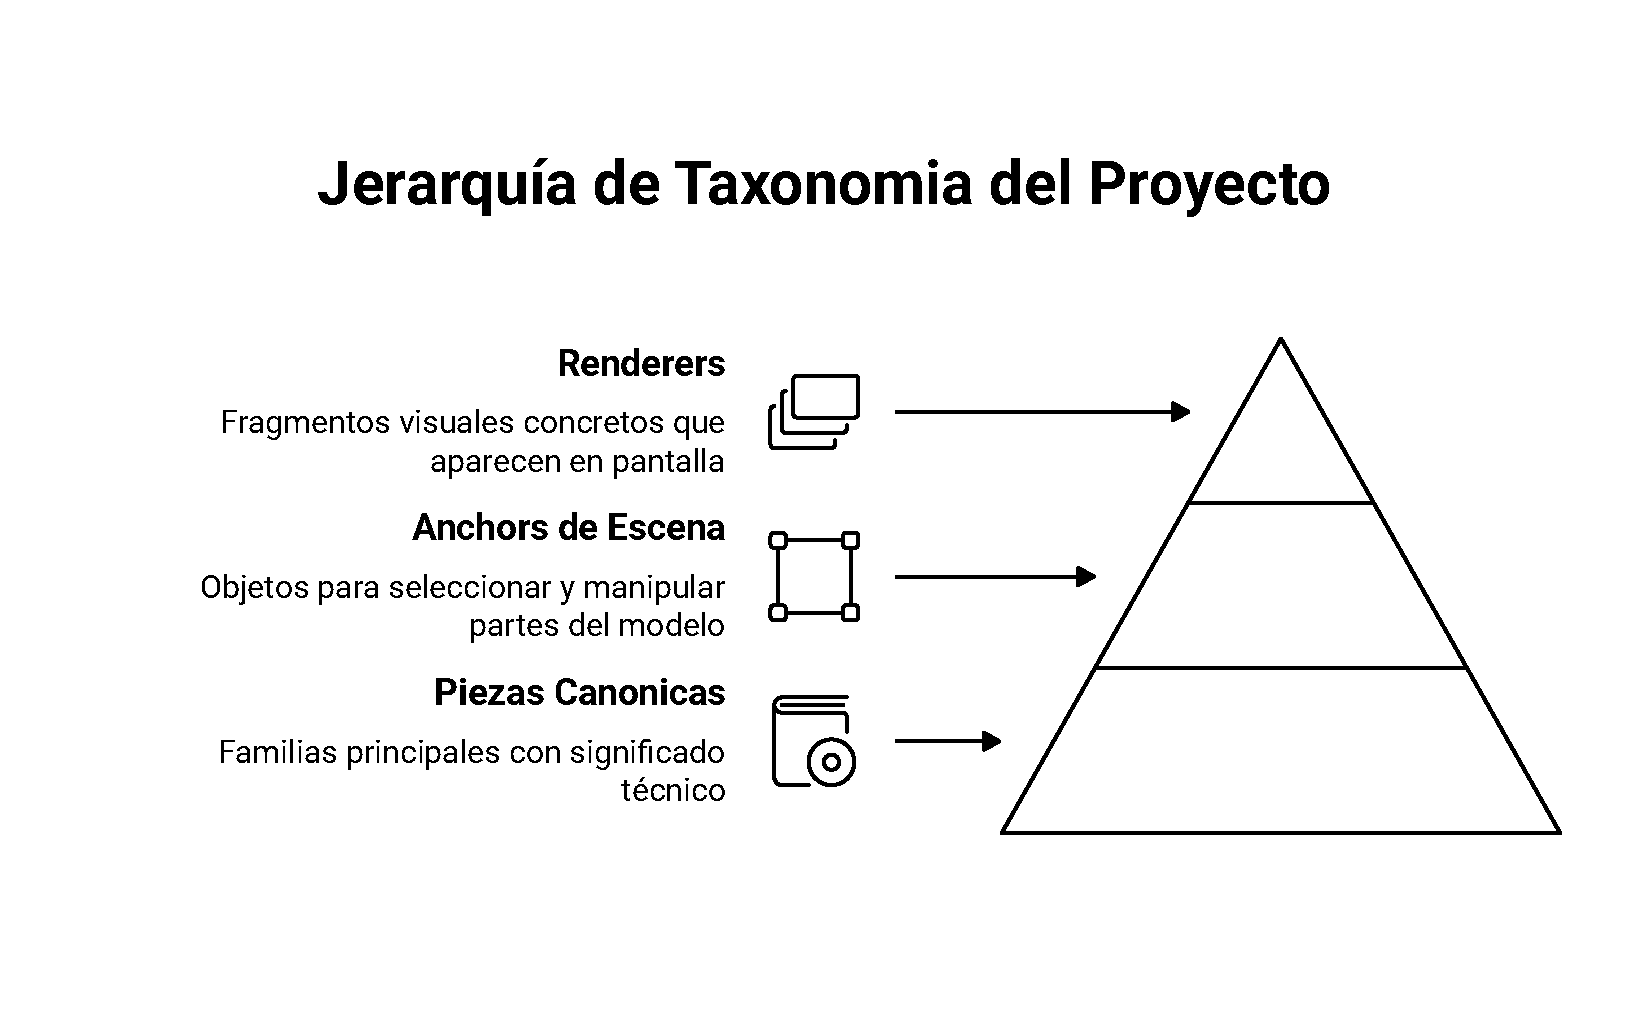
\includegraphics[width=0.88\textwidth,height=0.58\textheight,keepaspectratio]{figures/chapter4/fig_4_taxonomia_28_30_257.pdf}
    \par\vspace{0.5\baselineskip}
    \apanote{Mapeo jerárquico que organiza las 28 piezas canónicas de la investigación en 30 anchors de escena en Unity y 257 renderers y colliders físicos en runtime. Elaboración propia.}
\end{figure}

\subsection{Evolución del proyecto y consolidación del caso de estudio}

El desarrollo del prototipo atravesó varias reformulaciones antes de llegar al estado actual. En una fase inicial, el producto se entendía como un visor 3D con pocas piezas funcionales y fuerte énfasis en la arquitectura de interacción. Más adelante, el proyecto se desplazó hacia un caso de estudio técnicamente más exigente: el dron Holybro X500~V2 como ejemplo de \textit{hardware complejo}, entendido aquí como un sistema electromecánico multicomponente con integración estructural, energética, electrónica y de control, alta densidad de relaciones espaciales entre piezas y necesidad de inspección visual del ensamblaje.

Ese cambio de foco alteró tanto la producción de activos como la app (véase la Tabla \ref{tab:hitos_desarrollo_proyecto}). La transición implicó abandonar una lectura reducida del sistema, ampliar la taxonomía, reestructurar la escena, redefinir el flujo de selección y replantear la interfaz desde una lógica \textit{mobile-first}. También exigió separar lo ya visible en la build de lo que pertenece a legado técnico, funciones internas o cierre documental.

\subsubsection{Lectura del prototipo como visual product twin}

Desde el cierre conceptual del proyecto, el producto se entiende como una capa de \textit{visual product twin}: una representación web 3D optimizada, navegable y semánticamente organizada del hardware, orientada a inspección, explicación técnica y preparación de datos. Esta lectura no cambia el alcance implementado, pero sí clarifica su valor industrial. La app final no sincroniza telemetría real ni ejecuta diagnóstico de mantenimiento; sin embargo, estabiliza identificadores visuales, categorías, grupos de escena, fichas, hotspots y herramientas de análisis que podrían mapearse en el futuro a sensores, procedimientos, eventos y repuestos.

En términos de madurez, la build publicada se ubica en el nivel de \textit{digital model} enriquecido: representa el producto con fidelidad visual y semántica, pero no recibe aún datos del activo físico. El siguiente paso lógico no sería declarar un gemelo digital completo, sino formalizar un \textit{twin manifest} independiente de Unity y conectar datos históricos o simulados que permitan reproducir estados por pieza. Esta progresión reduce riesgo técnico, evita sobrepromesas y mantiene coherencia con la literatura que distingue \textit{digital model}, \textit{digital shadow} y \textit{digital twin} (Kritzinger et al., 2018; Digital Twin Consortium, 2020). Los renderes finales del dron optimizado se reservan para el capítulo de resultados, donde se relacionan directamente con la reducción poligonal y el cierre visual del activo.

\begin{table}[H]
    \caption{Hitos de evolución técnica del desarrollo del proyecto}
    \label{tab:hitos_desarrollo_proyecto}
    \centering
    \small
    \begin{tabular}{p{2.8cm}p{4.0cm}p{2.6cm}p{5.0cm}}
        \hline
        \textbf{Etapa} & \textbf{Foco principal} & \textbf{Estado} & \textbf{Lectura para el informe} \\ \hline
        Prototipo temprano & Arquitectura base del visor y conteo reducido de piezas & Histórica & Explica el antecedente de ``16 piezas'', pero no representa el cierre documental. \\
        Consolidación del caso Holybro & Selección del X500~V2 y ampliación de taxonomía semántica & Ejecutado & Fija el marco real del proyecto y el cambio hacia \textit{hardware complejo}. \\
        Saneamiento de activos y escena & Reorganización de piezas, grupos sintéticos y reparación de runtime & Ejecutado & Sustenta la convención 28/30/257 y el flujo final de la app. \\
        Rediseño UI \textit{mobile-first} & Bottom sheet, navegación inferior, modos y responsive base & Ejecutado & Aporta la capa de diseño con respaldo teórico más fuerte del producto. \\
        Cierre técnico & Build WebGL, QA P1/P2, profiler interno y validación empírica & Build funcional y medición empírica & El flujo visible quedó validado para entrega; las mediciones formales se reportan con datos fechados de rendimiento y usuarios. \\ \hline
    \end{tabular}
    \par\vspace{0.5\baselineskip}
    \apanote{Esta tabla resume la evolución del proyecto y distingue cifras o decisiones tempranas frente al estado técnico vigente. Elaboración propia a partir del código, la documentación activa y la propuesta corregida.}
\end{table}

\subsection{Pipeline 3D, importación CAD y saneamiento geométrico}

El \textit{pipeline} de activos combinó ingeniería inversa visual, importación CAD, remodelado hard-surface, limpieza topológica, modularización de repetitivos y adaptación progresiva a un objetivo WebGL. El objetivo no fue conservar intacta la geometría de origen, sino traducirla a un activo navegable, seleccionable, explicable y desplegable en navegador bajo restricciones reales de memoria, \textit{draw calls} y presupuesto geométrico.

\subsubsection{Métodos de importación CAD y criterio de uso}

Durante el proyecto se estudiaron y utilizaron múltiples rutas de entrada para convertir información CAD en geometría útil para Blender y Unity. La importación directa fue útil para inspección rápida, apertura inicial o comparación de piezas, pero no constituyó la ruta de mayor calidad para producción. En la práctica, la selección entre Blender directo, STEPper, MoI3D, retopología, remodelado o proxies dependió del control de teselación, la limpieza de la malla, la criticidad visual y la viabilidad WebGL de cada familia geométrica (véanse la Tabla \ref{tab:metodos_importacion_cad} y la Figura \ref{fig:flujo_decision_cad_webgl}).

\begin{table}[p]
    \caption{Métodos de importación CAD considerados en el proyecto}
    \label{tab:metodos_importacion_cad}
    \centering
    \footnotesize
    \setlength{\tabcolsep}{3pt}
    \renewcommand{\arraystretch}{0.82}
    \begin{tabular}{>{\RaggedRight\arraybackslash}p{3.0cm}>{\RaggedRight\arraybackslash}p{3.25cm}>{\RaggedRight\arraybackslash}p{2.15cm}>{\RaggedRight\arraybackslash}p{4.85cm}}
        \hline
        \textbf{Ruta técnica} & \textbf{Uso principal} & \textbf{Estado} & \textbf{Interpretación} \\ \hline
        STEP $\rightarrow$ Blender directo & Inspección rápida de piezas y lectura geométrica inicial & Evaluado y usado de forma exploratoria & Útil para abrir piezas o familias sencillas, pero no siempre ofrece control suficiente sobre la teselación final. \\
        STEP $\rightarrow$ Blender mediante STEPper & Importación CAD directa dentro de Blender con apoyo de addon especializado & Ejecutado / evaluado & Aportó una ruta práctica para abrir archivos STEP sin salir del entorno de modelado, especialmente durante revisión, limpieza o comparación de piezas. \\
        STEP $\rightarrow$ MoI3D $\rightarrow$ exportación poligonal $\rightarrow$ Blender & Conversión de superficies NURBS/CAD con control más fino de salida & Ejecutado & Se utilizó para casos donde la importación directa producía mallas difíciles de reutilizar o inconsistentes en topología. \\
        Re-modelado sobre referencia CAD en Blender & Reconstrucción de piezas con topología defendible para tiempo real & Ejecutado & Fue la ruta dominante para piezas críticas, especialmente cuando la malla de origen no era apta para WebGL. \\
        Sustitución modular de repetitivos & Tornillería, arandelas y elementos similares de alta repetición & Ejecutado & Redujo redundancia geométrica y abrió la puerta a instanciación, familias y proxies ligeros. \\ \hline
    \end{tabular}
    \par\vspace{0.5\baselineskip}
    \apanote{La coexistencia de varias rutas refleja la necesidad de adaptar el pipeline a distintos tipos de geometría CAD. Elaboración propia.}
\end{table}

\begin{figure}[htbp]
    \caption{Flujo de decisión para importación y optimización CAD a WebGL.}
    \label{fig:flujo_decision_cad_webgl}
    \centering
    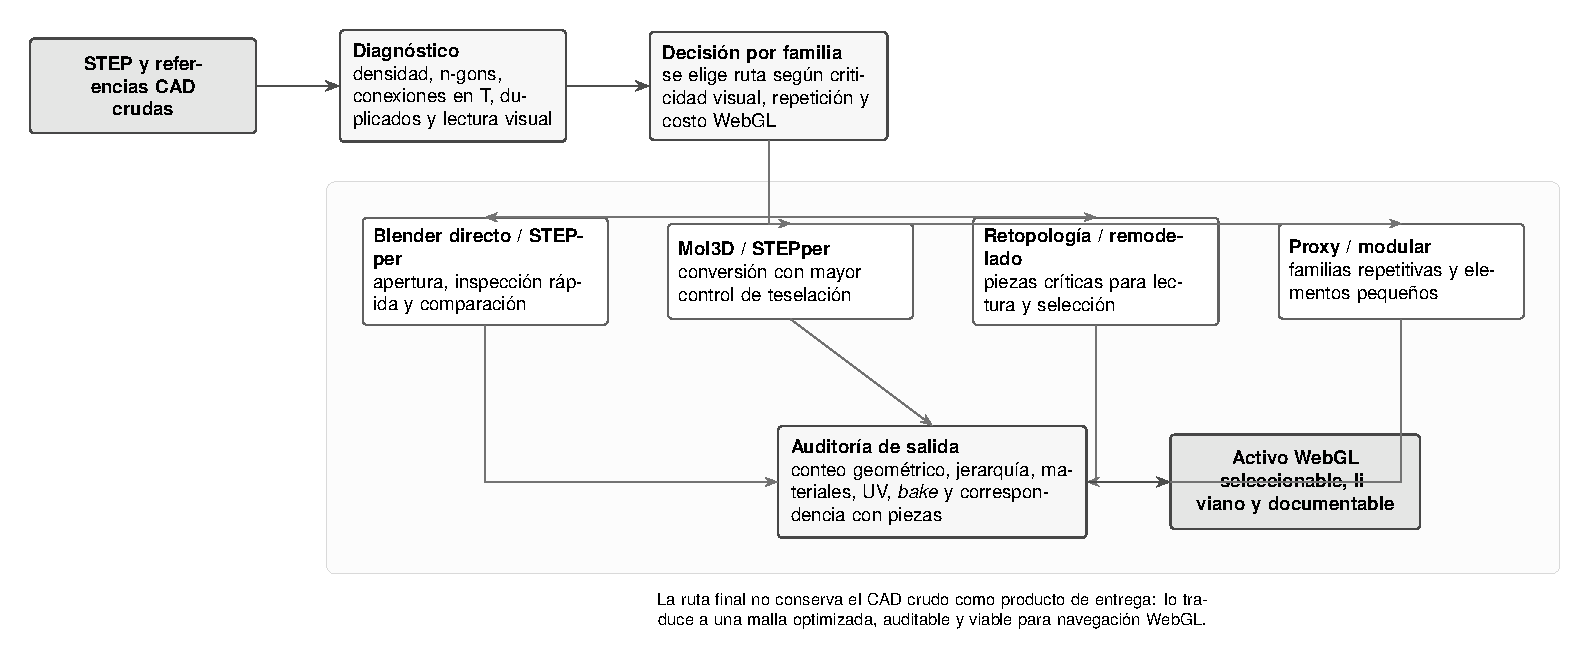
\includegraphics[width=0.92\textwidth,height=0.58\textheight,keepaspectratio]{figures/chapter4/fig_4_flujo_decision_cad_webgl.pdf}
    \par\vspace{0.5\baselineskip}
    \apanote{Rutas técnicas de importación evaluadas y ejecutadas para trasladar la geometría CAD a Blender y Unity, indicando criterios de optimización poligonal y control de teselación. Elaboración propia.}
\end{figure}

Las Figuras \ref{fig:cad_importacion_directa_step_blender} y \ref{fig:cad_importacion_moi_ngons} complementan el flujo anterior con evidencia visual de dos rutas de entrada al pipeline. En ambos casos se muestra la vista sombreada junto a su lectura \textit{wireframe}, porque el problema técnico no se limita a la apariencia externa del dron, sino a la estructura de la malla que luego debe limpiarse, triangularse u optimizarse.

\begin{figure}[htbp]
    \caption{Importación directa STEP a Blender con vista sombreada y \textit{wireframe}.}
    \label{fig:cad_importacion_directa_step_blender}
    \centering
    \includegraphics[width=\textwidth,height=0.54\textheight,keepaspectratio]{figures/screenshots_contextual/fig_cad_just_imported_pair.png}
    \par\vspace{0.5\baselineskip}
    \apanote{A la izquierda se observa el modelo importado de forma directa desde STEP a Blender; a la derecha se presenta su equivalente en \textit{wireframe}. Elaboración propia.}
\end{figure}

\begin{figure}[htbp]
    \caption{Importación desde MoI3D sin triangulación final con vista sombreada y \textit{wireframe}.}
    \label{fig:cad_importacion_moi_ngons}
    \centering
    \includegraphics[width=\textwidth,height=0.54\textheight,keepaspectratio]{figures/screenshots_contextual/fig_cad_ngons_pair.png}
    \par\vspace{0.5\baselineskip}
    \apanote{A la izquierda se muestra el modelo convertido desde MoI3D sin triangular; a la derecha se evidencia la presencia de n-gons y estructura de malla que requiere saneamiento antes del uso en WebGL. Elaboración propia.}
\end{figure}

\subsubsection{MAD-T como marco técnico adaptado para activos hard-surface WebGL}

Como referencia de producción hard-surface se adoptó de manera adaptada el marco MAD-T divulgado por Blender Bros, asociado a las operaciones de \textit{Modeling, Automation, Decimation} y \textit{Triangulation} (Blender Bros, 2022). En su contexto original, MAD-T funciona como un flujo práctico para preparar mallas hard-surface de tiempo real: primero se resuelve la forma del objeto, luego se automatizan operaciones técnicas repetitivas sobre aristas, costuras y superficies, después se reduce la complejidad geométrica y finalmente se triangula de forma explícita para cerrar una malla estable.

En este proyecto, MAD-T no se usó como metodología académica ni como receta cerrada. Se utilizó como criterio técnico de producción dentro del pipeline CAD--Blender--Unity, porque el punto de partida no era un asset de videojuego modelado desde cero, sino geometría CAD heterogénea del Holybro X500~V2. Esa diferencia obligó a adaptar cada fase según el estado real de las piezas.

\begin{itemize}
    \item \textbf{Modeling.} La fase de modelado no consistió únicamente en remodelar sobre referencia CAD. Dependiendo de la pieza, se siguieron tres rutas: piezas inexistentes que debieron modelarse desde cero; piezas existentes cuya malla CAD convertida no era trabajable y requirió retopología (véase la Figura \ref{fig:retopologia_pipeline}); y piezas que conservaron su geometría base, pero necesitaron correcciones puntuales por problemas típicos de conversión STEP a malla, como vértices no soldados, vértices repetidos, conexiones poligonales en T, caras internas, normales inconsistentes, geometría suelta o triangulaciones inestables.
    \item \textbf{Automation.} Esta fase conservó el sentido técnico del MAD-T original: reducir trabajo repetitivo mediante herramientas y operaciones automatizables sobre la malla. En el proyecto incluyó selección de aristas duras, tratamiento de bevels generales, control de costuras, limpieza de marcas problemáticas, normalización de bordes, uso de modificadores y preparación consistente de superficies hard-surface antes de la reducción y exportación.
    \item \textbf{Decimation.} La reducción geométrica se aplicó cuando el detalle no aportaba legibilidad técnica o excedía el presupuesto esperado para WebGL. La decisión no fue eliminar detalle de forma indiscriminada, sino conservar silueta, lectura funcional y relaciones de ensamblaje mientras se disminuía el costo de vértices y triángulos.
    \item \textbf{Triangulation.} La triangulación se entendió como cierre de producción: una forma de evitar que Blender, el importador de Unity o el runtime WebGL decidieran triangulaciones implícitas distintas. Esto permitió estabilizar sombreado, normales, UVs y comportamiento de exportación.
\end{itemize}

Así, MAD-T operó como una capa de saneamiento y preparación de activos hard-surface (véase la Tabla \ref{tab:trazabilidad_familias_pipeline}), mientras que la metodología académica del proyecto se mantuvo en el diseño, implementación y evaluación del artefacto interactivo (véase la Figura \ref{fig:madt_adaptado_pipeline}).

\begin{figure}[htbp]
    \caption{Adaptación del flujo MAD-T al pipeline CAD--WebGL del proyecto.}
    \label{fig:madt_adaptado_pipeline}
    \centering
    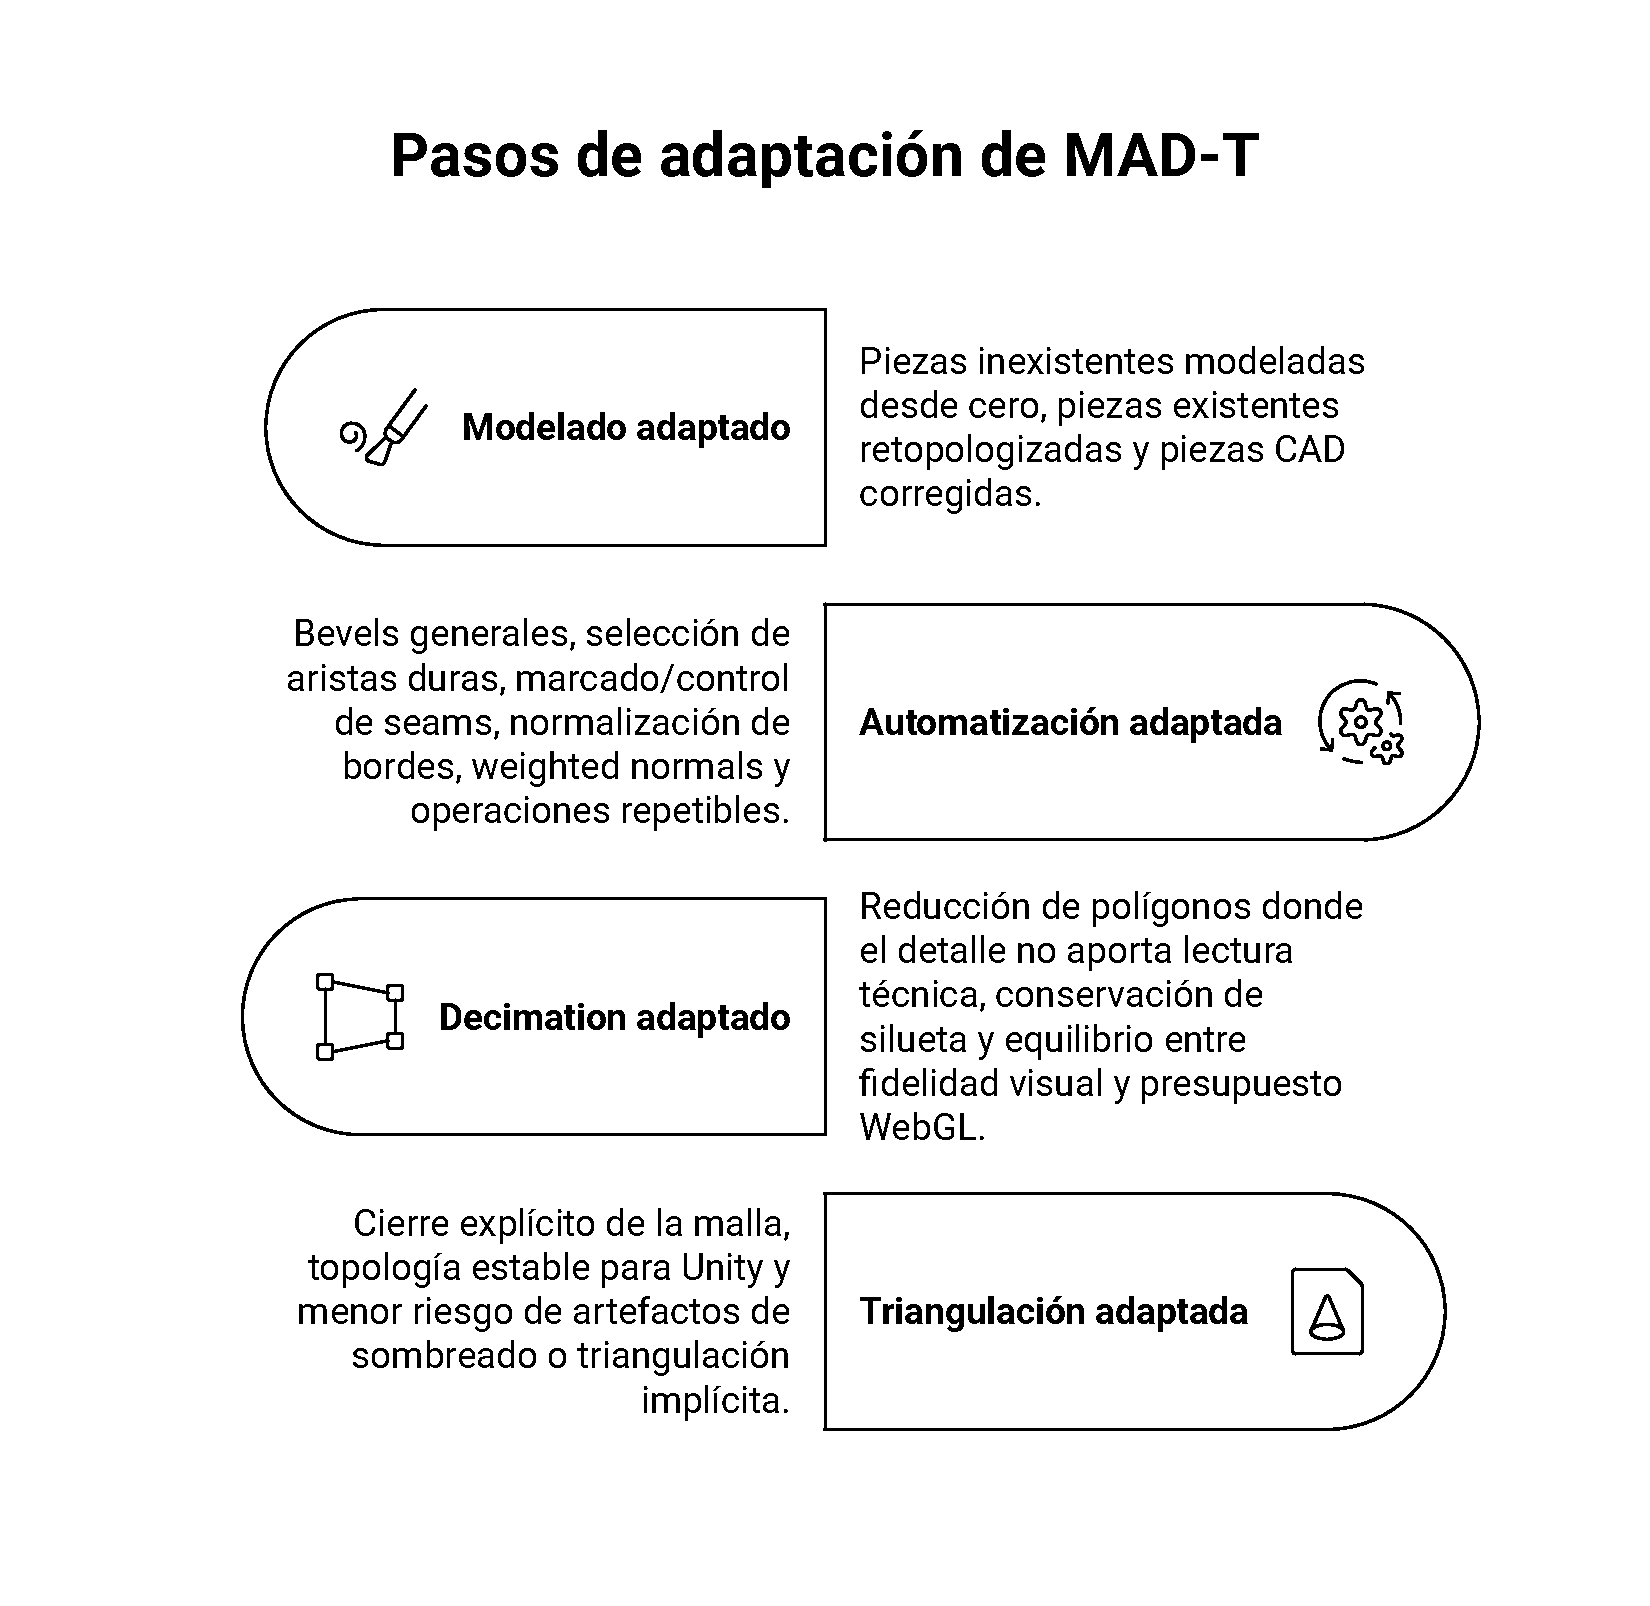
\includegraphics[width=0.86\textwidth,height=0.58\textheight,keepaspectratio]{figures/chapter4/fig_4_madt_adaptado.pdf}
    \par\vspace{0.5\baselineskip}
    \apanote{La adaptación se usó como criterio técnico de producción hard-surface; no reemplaza la metodología académica DSRM del proyecto. Elaboración propia.}
\end{figure}

\begin{table}[H]
    \caption[Trazabilidad CAD--runtime]{Trazabilidad representativa entre familia CAD, acción aplicada y salida runtime}
    \label{tab:trazabilidad_familias_pipeline}
    \centering
    \scriptsize
    \setlength{\tabcolsep}{3pt}
    \begin{tabular}{p{3.0cm}p{3.8cm}p{4.1cm}p{4.3cm}}
        \hline
        \textbf{Familia o pieza} & \textbf{Entrada o referencia principal} & \textbf{Acción aplicada} & \textbf{Salida runtime o canónica} \\ \hline
        Placas del frame & Piezas CAD del kit X500 (\texttt{BOTTOM-PLATE}, \texttt{TOP-PLATE}, \texttt{PLATFORM-PLAT}) & Limpieza, renombrado y adaptación para escena. & Anchors canónicos \texttt{x500v2\_bottom\_plate}, \texttt{x500v2\_top\_plate} y \texttt{x500v2\_platform\_board}. \\
        Brazos y soportes de motor & Tubo de carbono, montajes y clamps del frame. & Agrupación por familia e instanciación por cuadrante para conservar simetría y reducir trabajo manual. & Anchors \texttt{x500v2\_arm\_FL/FR/BL/BR}. \\
        Pixhawk 6C & Carcasa, PCB e IMU separados en CAD o referencia técnica. & Encapsulado de subpiezas en una lectura semántica única para la ficha técnica. & Anchor \texttt{x500v2\_pixhawk6c}. \\
        GPS M10 & Antena, mástil, base, bandeja y tuerca. & Unión semántica de subpartes y normalización de nombres para selección y documentación. & Anchor \texttt{x500v2\_gps\_m10}. \\
        Motores & Modelo base de motor y réplica por cuadrante. & Instanciación del modelo base y asignación a las posiciones funcionales del dron. & Anchors \texttt{x500v2\_motor\_FL/FR/BL/BR}. \\
        ESC, hélices, batería y radio & Manuales, referencias CAD parciales y proxies de trabajo. & Modelado o proxy según disponibilidad de referencia, importancia visual y tiempo disponible. & Nodos canónicos con cobertura suficiente para lectura del ensamblaje. \\
        Fasteners repetitivos & Familias CAD GB70 y sujetadores repetidos del frame. & Clasificación semántica, proxies ligeros y reemplazo modular delimitado a tornillos. & Grupo \texttt{x500v2\_fastener\_group} con metadatos de familia en runtime. \\ \hline
    \end{tabular}
    \par\vspace{0.5\baselineskip}
    \apanote{La tabla resume casos representativos y no pretende listar cada subpieza del pipeline. Su función es hacer auditable la relación entre fuente geométrica, operación aplicada y destino runtime. Elaboración propia a partir de inventarios internos del pipeline, escena Blender, catálogo runtime y revisión de correspondencia CAD--Unity.}
\end{table}

\subsubsection{Automatización propia en Blender: masters, instancias y proxies}

Además del uso adaptado de MAD-T, el proyecto requirió tooling propio dentro de Blender para resolver un problema específico de los ensambles CAD: muchas piezas repetidas llegan como objetos independientes, con transformaciones horneadas en los vértices, orígenes globales inconsistentes o mallas duplicadas que impiden aprovechar instancias reales. Esto afecta rendimiento, mantenimiento, retopología, bake de texturas y animaciones como la vista explosionada.

Para ordenar este flujo se distinguieron tres conceptos operativos:
\begin{itemize}
    \item \textbf{Master.} Malla limpia o saneada que funciona como referencia geométrica compartida de una familia repetida. Un master puede servir solo como fuente técnica para instancias o coincidir con una ocurrencia visible del ensamblaje cuando esa pieza también existe físicamente en el dron.
    \item \textbf{Instancia.} Objeto que comparte datos de malla con un master, pero conserva transformación, posición, rotación y escala propias dentro del ensamblaje. Esto permite corregir una sola malla y propagar el cambio a todas sus ocurrencias.
    \item \textbf{Proxy.} Representación geométrica ligera usada cuando una pieza no requiere detalle completo en reposo o cuando una familia repetitiva sería demasiado costosa si se conservara con su malla CAD original. El proxy conserva lectura morfológica y posición espacial, pero reduce vértices, peso y costo de inspección.
\end{itemize}

Esta separación permitió que el pipeline no dependiera de colapsar todo el modelo ni de destruir la estructura del ensamblaje. En cambio, se conservaron relaciones entre piezas físicas, instancias repetidas, geometría liviana y metadatos exportables hacia Unity. Para hacer auditable la exportación, el pipeline generó un manifest de Blender con roles, matrices de transformación, límites espaciales, relación master/instancia y candidatos de asociación entre fasteners y pieza madre. Este manifest no reemplazó la revisión manual cuando había ambigüedad, pero redujo la posibilidad de importar una escena sin trazabilidad hacia Unity (véase la Figura \ref{fig:automatizacion_blender_masters_instancias}). Los criterios usados para comparar el saneamiento geométrico se resumen en la Tabla \ref{tab:comparativa_saneamiento_geometrico_cap4}; las cifras medidas corresponden al análisis de resultados.

\begin{figure}[htbp]
    \caption{Tooling propio en Blender para masters, instancias, proxies y manifest.}
    \label{fig:automatizacion_blender_masters_instancias}
    \centering
    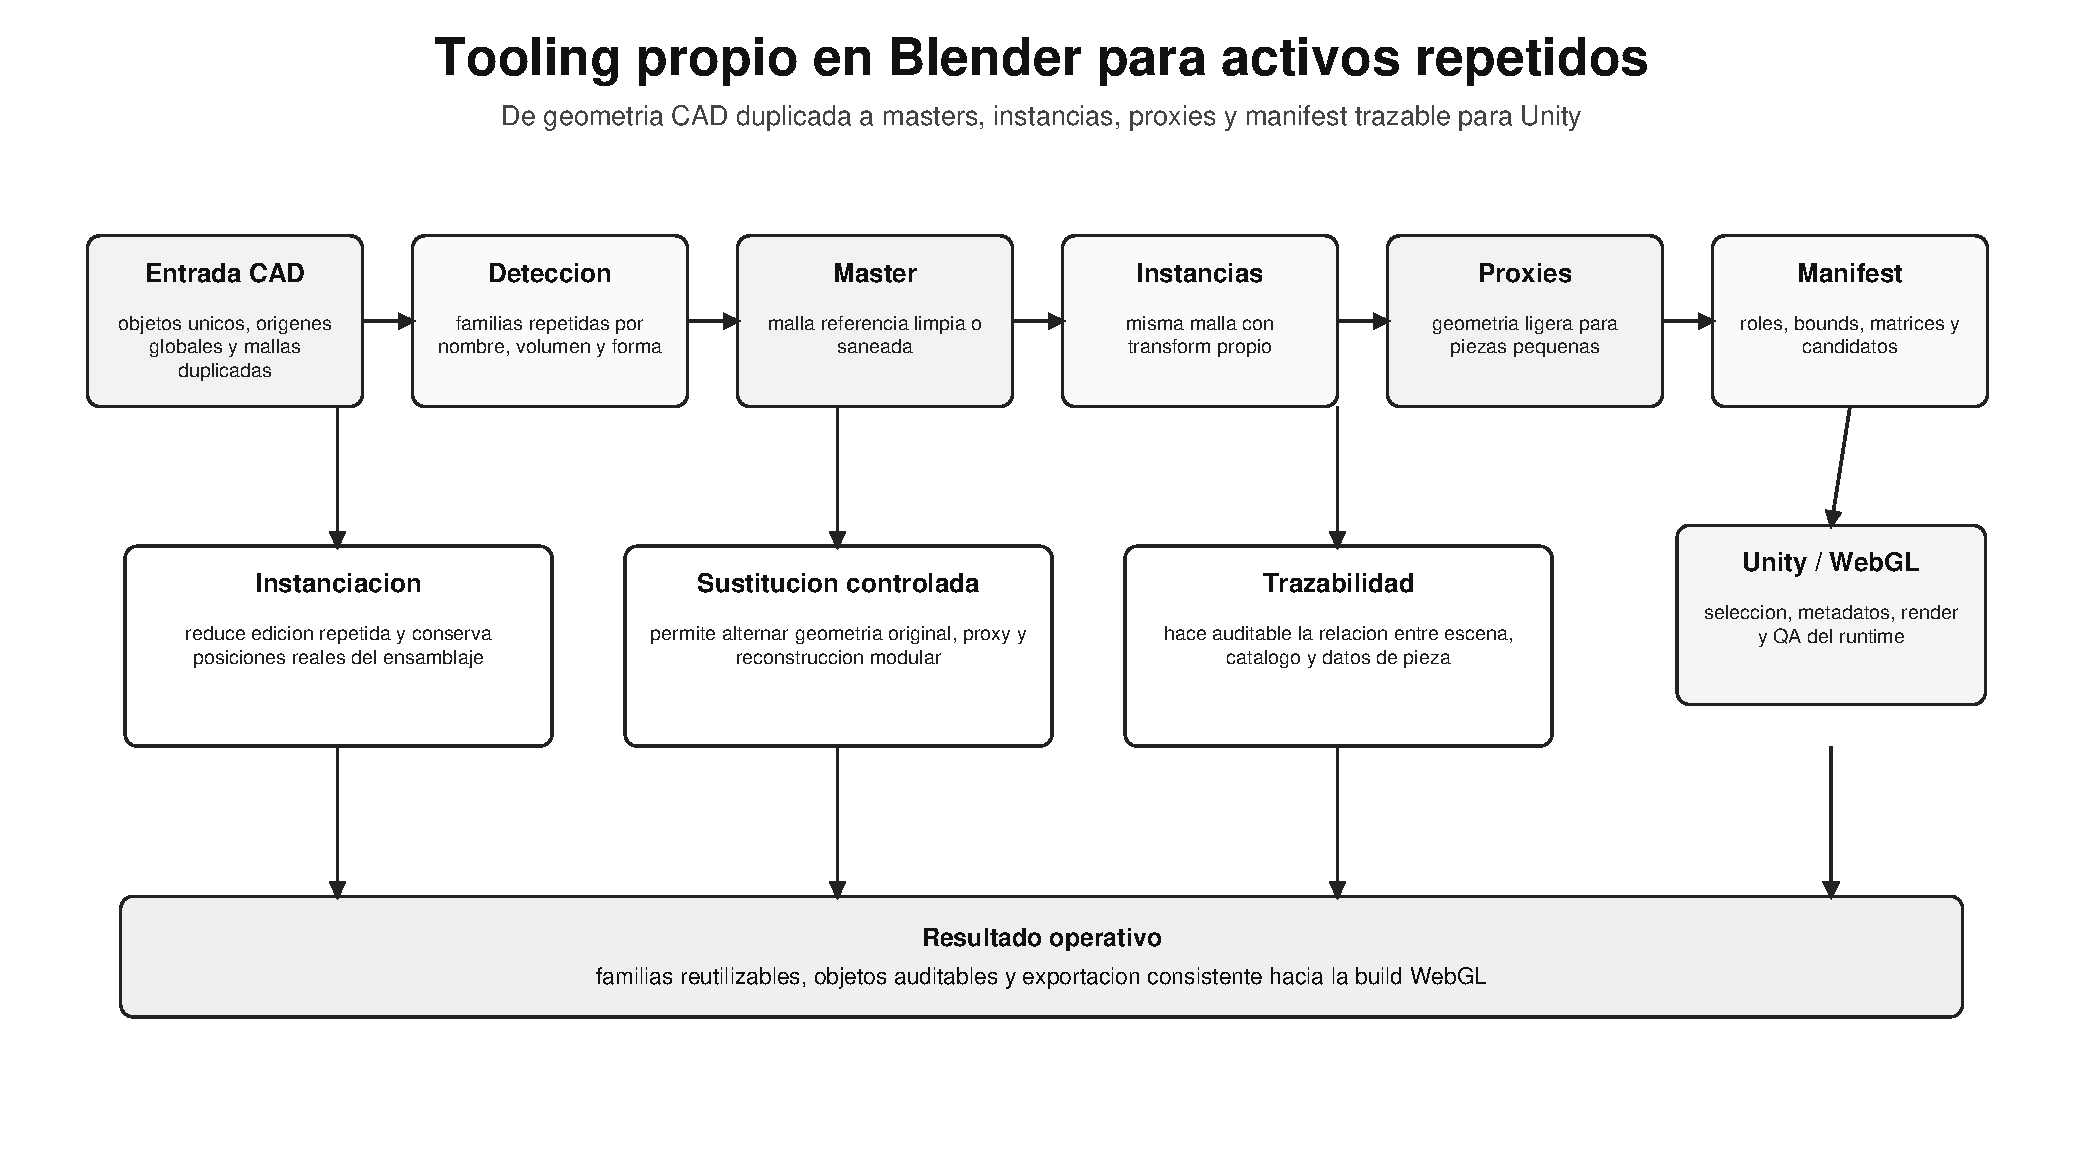
\includegraphics[width=\textwidth,height=0.52\textheight,keepaspectratio]{figures/chapter4/fig_4_automatizacion_blender_masters_instancias.pdf}
    \par\vspace{0.5\baselineskip}
    \apanote{La figura muestra herramientas de preparación de activos; no corresponde a funciones visibles de la app final para usuarios. Elaboración propia.}
\end{figure}

\begin{figure}[htbp]
    \caption{Saneamiento de geometría CAD para runtime WebGL.}
    \label{fig:retopologia_pipeline}
    \centering
    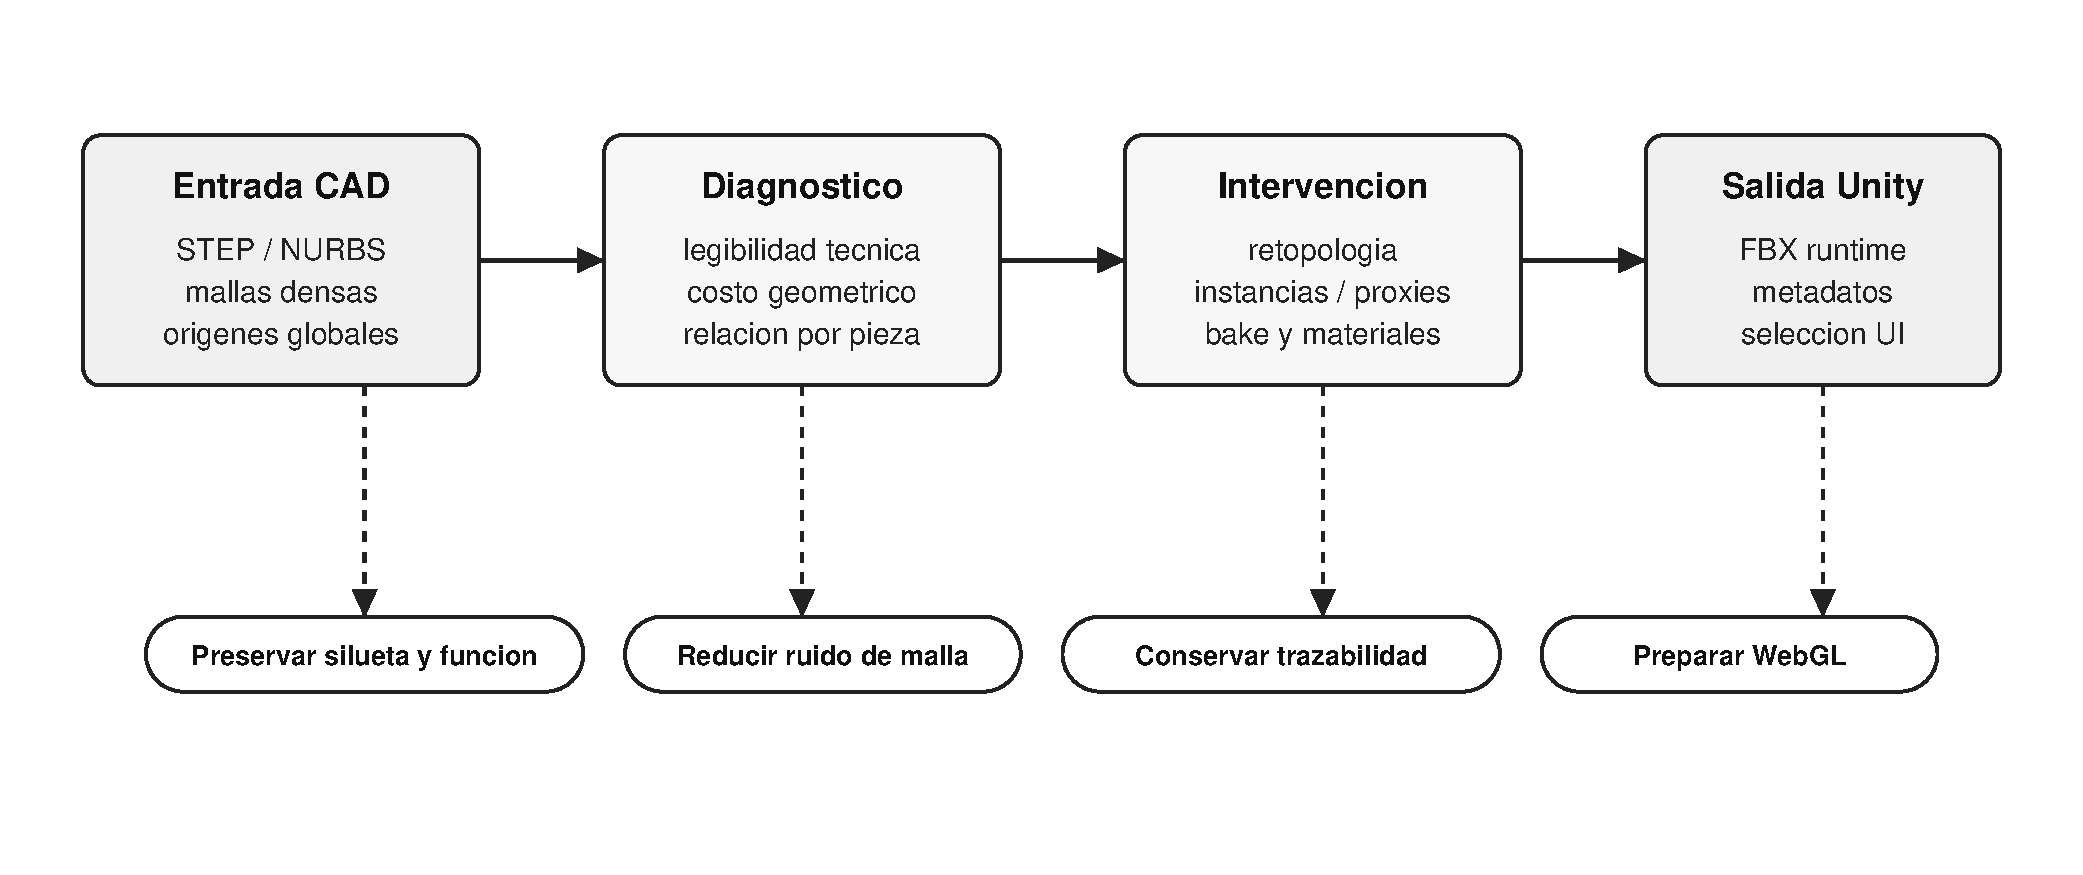
\includegraphics[width=\textwidth,height=0.58\textheight,keepaspectratio]{figures/chapter4/fig_4_retopologia_pipeline.pdf}
    \par\vspace{0.5\baselineskip}
    \apanote{Diagrama conceptual del flujo de saneamiento geométrico aplicado para transformar geometría CAD en activos aptos para runtime WebGL. Elaboración propia.}
\end{figure}

\begin{table}[p]
    \caption{Criterios para comparar el saneamiento geométrico}
    \label{tab:comparativa_saneamiento_geometrico_cap4}
    \centering
    \footnotesize
    \setlength{\tabcolsep}{3pt}
    \renewcommand{\arraystretch}{0.86}
    \begin{tabular}{>{\RaggedRight\arraybackslash}p{3.2cm}>{\RaggedRight\arraybackslash}p{3.6cm}>{\RaggedRight\arraybackslash}p{6.5cm}}
        \hline
        \textbf{Familia o caso} & \textbf{Métrica de comparación} & \textbf{Lectura técnica} \\ \hline
        Brazo o soporte crítico & Triángulos, vértices y estabilidad de normales. & Permite contrastar la geometría de origen frente a una versión apta para runtime sin perder silueta funcional. \\
        Motor o carcasa compleja & Instancias, limpieza de malla y continuidad de sombreado. & Muestra cuándo conviene conservar, limpiar o reconstruir una pieza según su visibilidad e impacto en rendimiento. \\
        Fasteners repetitivos & Cantidad de instancias, familias y sustitución por proxy. & Evidencia el ahorro geométrico y semántico obtenido al agrupar sujetadores repetidos. \\
        Ensamble o subsistema representativo & Costo geométrico agregado y legibilidad del ensamblaje. & Relaciona el saneamiento con presupuesto WebGL, selección por pieza y comprensión visual del sistema. \\ \hline
    \end{tabular}
    \par\vspace{0.5\baselineskip}
    \apanote{La tabla define qué se compara; los valores cuantitativos se reportan en el capítulo de resultados con evidencia de la build evaluada. Elaboración propia.}
\end{table}

\subsubsection{Sistema modular de tornillería y ahorro geométrico}

Uno de los problemas más costosos del pipeline fue la tornillería. Los modelos CAD tienden a repetir pernos, tuercas, arandelas y sujetadores como mallas únicas, aunque geométrica y funcionalmente pertenezcan a familias repetidas. Si esa estructura se conserva sin filtrar, se dispara el costo en vértices, \textit{draw calls}, inspección y mantenimiento.

La respuesta del proyecto fue construir una capa modular para fasteners. En lugar de documentar cada tornillo como pieza semántica independiente, se organizaron \textbf{familias} reutilizables, \textbf{instancias} ubicadas en la escena y \textbf{entradas de reconciliación} para resolver diferencias de nombre entre Blender, catálogos y Unity. Una familia es el tipo reutilizable de sujetador, por ejemplo un tornillo de una métrica y forma de cabeza determinadas. Una instancia es una ocurrencia concreta de esa familia en el ensamblaje, con posición, rotación y relación espacial propia. Una entrada de reconciliación es el puente que permite asociar nombres cuando el objeto exportado desde Blender, el catálogo técnico y el identificador leído por Unity no coinciden literalmente. En la escena documentada quedaron versionadas \textbf{20 familias}, \textbf{168 instancias} y \textbf{9} entradas de reconciliación. Este trabajo alivió el presupuesto geométrico y permitió que el \textit{runtime} mostrara metadatos de familia, métrica, longitud, material y anclaje sin duplicar la lógica por instancia (como se detalla en la Tabla \ref{tab:fasteners_modulares_runtime} y se ilustra en las Figuras \ref{fig:fasteners_modular_pieces} y \ref{fig:fasteners_modular_array}).

En este contexto, la optimización de fasteners tuvo dos niveles. El primero fue semántico: agrupar familias, registrar instancias y reconciliar nombres entre Blender, catálogos y Unity. El segundo fue geométrico: decidir cuándo conservar geometría original, cuándo usar proxies ligeros y cuándo aplicar reemplazo modular. En la versión de cierre, el sistema modular se implementó únicamente en tornillos. Otros elementos pequeños, como tuercas, standoffs, grommets o arandelas, quedaron resueltos caso por caso: algunos conservaron geometría original y otros usaron proxies ligeros cuando su detalle no aportaba información relevante para la inspección visual.

\begin{table}[H]
    \caption{Lectura técnica del sistema modular de fasteners}
    \label{tab:fasteners_modulares_runtime}
    \centering
    \small
    \begin{tabular}{p{3.4cm}p{2.6cm}p{6.8cm}}
        \hline
        \textbf{Componente} & \textbf{Magnitud} & \textbf{Función en el proyecto} \\ \hline
        Familias de fasteners & 20 & Agrupan sujetadores equivalentes para evitar tratarlos como objetos aislados y permitir metadatos compartidos por tipo. \\
        Instancias registradas & 168 & Conservan la ubicación de cada ocurrencia concreta dentro del ensamblaje y permiten asociarla con una familia. \\
        Entradas de reconciliación & 9 & Resuelven diferencias entre nombres de escena, catálogo y metadatos para que Unity pueda recuperar la lectura correcta. \\
        Reemplazo modular & Tornillos & Se aplicó como caso cerrado de reconstrucción modular y ahorro geométrico; otros fasteners se resolvieron mediante geometría original o proxies ligeros según su relevancia visual. \\ \hline
    \end{tabular}
    \par\vspace{0.5\baselineskip}
    \apanote{La modularización de fasteners integra datos, escena y optimización; no se limita a una agrupación visual. Elaboración propia a partir de la escena y del runtime de fasteners del proyecto.}
\end{table}

La Figura \ref{fig:fasteners_modular_pieces} muestra las piezas base del sistema modular de tornillos. Estas cinco piezas permiten variar cabeza, diámetro, densidad vertical y longitud mediante repetición controlada del cuerpo. La Figura \ref{fig:fasteners_modular_array} muestra un ejemplo de tornillo generado con una cabeza y un arreglo de siete segmentos de cuerpo.

\begin{figure}[htbp]
    \caption{Piezas base del sistema modular de tornillos.}
    \label{fig:fasteners_modular_pieces}
    \centering
    \includegraphics[width=\textwidth,height=0.42\textheight,keepaspectratio]{figures/screenshots_contextual/fig_fastener_modular_pieces.png}
    \par\vspace{0.5\baselineskip}
    \apanote{La reconstrucción modular de tornillos se basa en combinaciones de cabeza, diámetro y segmentos de cuerpo para ajustar longitud sin conservar una malla CAD única por cada tornillo. Elaboración propia.}
\end{figure}

\begin{figure}[htbp]
    \caption{Ejemplo de tornillo generado mediante arreglo modular.}
    \label{fig:fasteners_modular_array}
    \centering
    \includegraphics[width=0.82\textwidth,height=0.48\textheight,keepaspectratio]{figures/screenshots_contextual/fig_fastener_modular_array.png}
    \par\vspace{0.5\baselineskip}
    \apanote{El ejemplo muestra un tornillo compuesto por una cabeza y siete segmentos repetidos de cuerpo, lo que ilustra el principio de variación de longitud mediante arreglo. Elaboración propia.}
\end{figure}

\begin{figure}[htbp]
    \caption{Sistema modular delimitado a tornillos y reconciliación de fasteners.}
    \label{fig:pipeline_modular_screw_only}
    \centering
    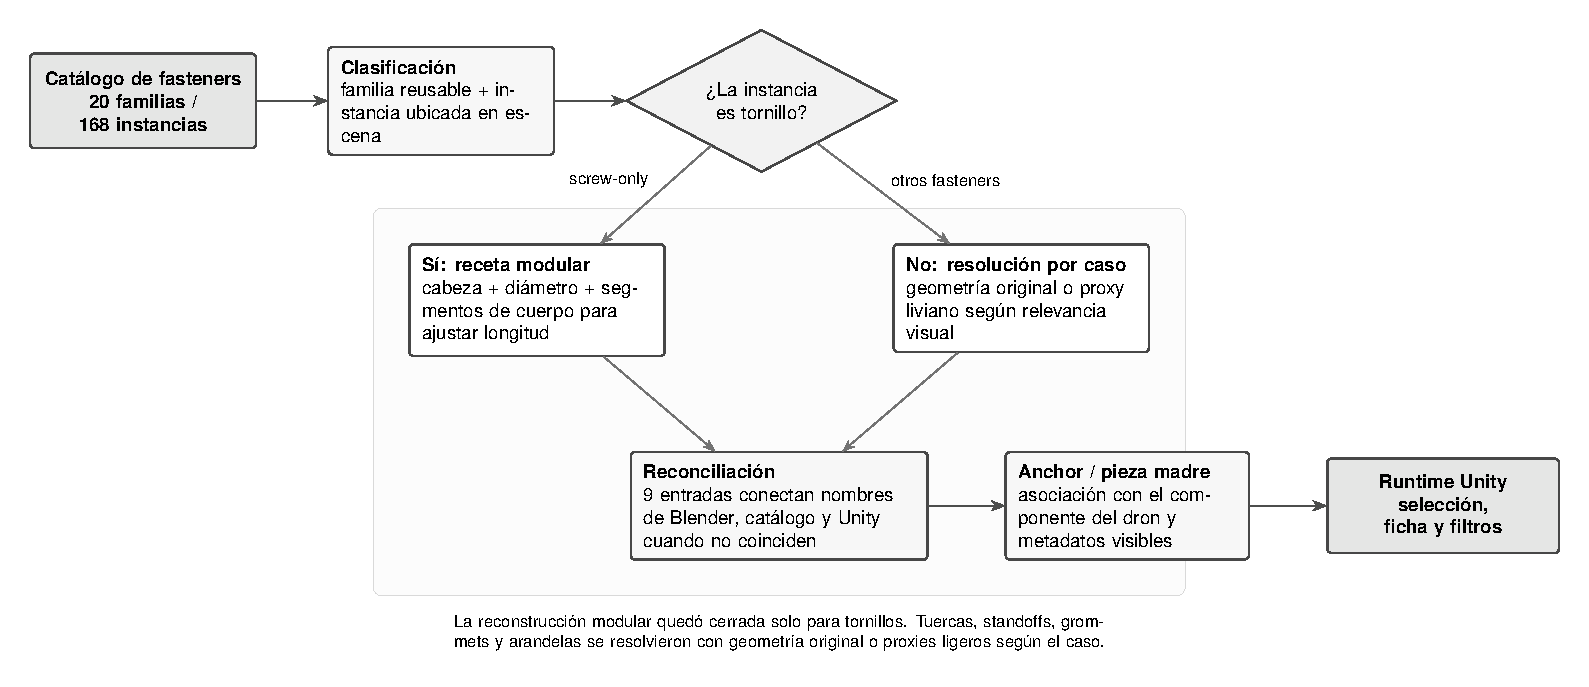
\includegraphics[width=0.96\textwidth,height=0.58\textheight,keepaspectratio]{figures/chapter4/fig_4_pipeline_modular_screw_only.pdf}
    \par\vspace{0.5\baselineskip}
    \apanote{El diagrama distingue la reconstrucción modular aplicada solo a tornillos de la resolución por caso usada para otros fasteners, ya sea con geometría original o proxies ligeros. Elaboración propia.}
\end{figure}

En el flujo Blender--Unity, la escena runtime se exporta como unión de cuatro colecciones: masters bakeados, instancias del ensamblaje, masters primitivos de fasteners e instancias primitivas de fasteners. La decisión de exportar un master depende de su papel en el ensamblaje: puede ser solo referencia geométrica compartida o una ocurrencia visible que también debe aparecer en la escena final. El paquete de materiales previsto usa \texttt{BaseColor}, \texttt{Normal} y una máscara compacta \texttt{R=AO}, \texttt{G=Roughness}, \texttt{B=Curvature}, \texttt{A=Metallic}; la fibra de carbono se hornea desde el material construido en Blender. La asignación de fasteners a piezas madre se trata como revisión basada en manifest y no como inferencia automática cuando exista ambigüedad. El reemplazo modular queda limitado a tornillos; aplicar la misma reconstrucción a otros sujetadores se conserva como mejora futura del pipeline.

La Figura \ref{fig:fasteners_originales_y_proxies} compara fasteners originales frente a proxies recortados generados con el addon y primitivas básicas. Esta evidencia visual no implica que todos los sujetadores hayan sido reconstruidos modularmente: documenta la coexistencia entre geometría original, proxies ligeros y reconstrucción modular aplicada solo a tornillos.

\begin{figure}[htbp]
    \caption{Fasteners originales y proxies ligeros usados en el pipeline.}
    \label{fig:fasteners_originales_y_proxies}
    \centering
    \makebox[\textwidth][c]{\includegraphics[width=0.96\textwidth,height=0.68\textheight,keepaspectratio]{figures/screenshots_contextual/fig_fastener_original_proxy_stack.png}}
    \par\vspace{0.5\baselineskip}
    \apanote{La franja superior presenta fasteners en su forma original; la franja inferior muestra proxies ligeros generados con primitivas básicas y apoyo del addon. Elaboración propia.}
\end{figure}

\subsubsection{Software especializado y costo del pipeline}

La producción de activos combinó software libre, herramientas comerciales especializadas y addons de Blender. La Tabla \ref{tab:software_pipeline_3d} no busca fijar precios exactos, sino documentar las dependencias del pipeline y su nivel relativo de costo, ya que las licencias varían por versión, región y plan.

\clearpage

\begin{table}[htbp]
    \caption{Software y addons del pipeline 3D}
    \label{tab:software_pipeline_3d}
    \centering
    \scriptsize
    \setlength{\tabcolsep}{2pt}
    \begin{tabular}{p{2.0cm}p{2.55cm}p{2.0cm}p{1.65cm}p{3.15cm}}
    \hline
    \textbf{Herramienta} & \textbf{Rol principal} & \textbf{Licencia} & \textbf{Rango} & \textbf{Interpretación} \\ \hline
    Blender & Modelado, limpieza, organización y exportación & Libre / gratuita & Sin costo directo & Núcleo ejecutado del pipeline de producción. \\
    Unity & Integración, UI, shaders y despliegue web & Motor con plan de uso académico/personal & Sin costo directo en esta etapa & Punto de verdad del producto final. \\
    MoI3D & Conversión CAD y control de salida poligonal & Comercial especializada & Medio / alto & Usada como apoyo para piezas donde la teselación requería mayor control. \\
    STEPper & Importación de archivos STEP dentro de Blender & Addon especializado & Bajo / medio & Aportó una ruta directa para revisar, abrir o comparar piezas CAD sin salir del entorno de Blender. \\
    RizomUV & Despliegue y revisión UV para texturizado & Comercial especializada & Medio / alto & Apoyó la preparación de UVs cuando la geometría requería control más fino para texturas y bake. \\
    Hard Ops & Modelado hard-surface y booleans & Addon comercial & Bajo / medio & Complementó el re-modelado y la reconstrucción de piezas. \\
    Box Cutter & Corte rápido y booleans de precisión & Addon comercial & Bajo / medio & Aceleró iteraciones de remodelado y corrección. \\
    Mesh Machine & Limpieza de bevels y tratamiento hard-surface & Addon comercial & Bajo / medio & Se evaluó y aprovechó para limpieza de superficies duras y resolución de detalles. \\
    Marmoset Toolbag & Apoyo para bake/lookdev puntual & Comercial especializada & Medio / alto & Herramienta auxiliar del pipeline, no eje del runtime final. \\
    \hline
    \end{tabular}
    \par\vspace{0.5\baselineskip}
    \apanote{``Rango'' clasifica el tipo de inversión requerida sin fijar precios exactos sujetos a cambios comerciales. Elaboración propia a partir del pipeline del proyecto y de la investigación técnica asociada.}
\end{table}

La Figura \ref{fig:software_marmoset_rizomuv} documenta el uso de Marmoset Toolbag y RizomUV como herramientas auxiliares del pipeline de \textit{baking}, \textit{lookdev} y despliegue UV. Estas capturas se agrupan entre sí porque representan software especializado de preparación visual y texturizado, no estados de la app ni comparativas de importación CAD.

\begin{figure}[htbp]
    \caption{Software auxiliar para \textit{baking}, \textit{lookdev} y despliegue UV.}
    \label{fig:software_marmoset_rizomuv}
    \centering
    \includegraphics[width=\textwidth,height=0.68\textheight,keepaspectratio]{figures/screenshots_contextual/fig_software_marmoset_rizomuv.png}
    \par\vspace{0.5\baselineskip}
    \apanote{La captura superior corresponde a Marmoset Toolbag como apoyo de \textit{baking} y revisión visual; la inferior corresponde a RizomUV como herramienta de despliegue y revisión UV. Elaboración propia.}
\end{figure}

\subsubsection{Automatización y addons creados para el proyecto}

El volumen y la naturaleza de la geometría CAD hicieron inviable un flujo puramente manual. Por ello se desarrollaron y documentaron herramientas auxiliares para selección de piezas hermanas, instanciación, proxies, sustitución de mallas, preparación de bake y generación de manifests (cuyo resumen y funciones principales se describen en la Tabla \ref{tab:addons_automatizacion_pipeline} y se ilustran conceptualmente en la Figura \ref{fig:addons_pipeline_cad}).

El \textit{CAD Symmetry Instancer} se creó para detectar piezas repetidas, reconstruir relaciones de instancia y conservar transformaciones espaciales. Sus primeras versiones evidenciaron problemas propios de la geometría CAD importada: orígenes globales en el centro de la escena, rotaciones horneadas en vértices, simetrías radiales parciales y piezas cilíndricas donde técnicas como PCA podían producir giros ambiguos. Las versiones posteriores incorporaron estrategias más robustas, como validación por nombre, volumen, conteo de vértices, registro por matrices y variantes con ICP para casos de teselación irregular.

El \textit{CAD Mesh Swapper} resolvió otro problema frecuente: reemplazar la geometría interna de una pieza dañada por una versión limpia sin alterar su posición global. La herramienta permitía inyectar una malla saneada en un objeto objetivo y propagar el cambio a las instancias que compartían el mismo dato de malla, conservando materiales y transformaciones. En paralelo, el \textit{CAD Fastener Proxy Automator} se orientó a tornillería y repetitivos, analizando proporciones de cabezal y caña para generar proxies de baja complejidad con tipologías como socket, button o flat.

Finalmente, se desarrollaron scripts no destructivos para preparar el bake y la exportación final: creación de imágenes objetivo para mapas PBR, empaquetado de canales en máscaras runtime, y generación de un manifest de Blender con masters, instancias, roles, \textit{transforms}, \textit{bounds} y candidatos de pieza madre para fasteners. Estos scripts no sustituyeron la revisión manual, pero hicieron auditable el estado de la escena y redujeron el riesgo de exportar una jerarquía incompleta o ambigua.

\begin{table}[p]
    \caption{Automatizaciones y addons asociados al pipeline}
    \label{tab:addons_automatizacion_pipeline}
    \centering
    \footnotesize
    \setlength{\tabcolsep}{3pt}
    \renewcommand{\arraystretch}{0.72}
    \begin{tabular}{>{\RaggedRight\arraybackslash}p{2.65cm}>{\RaggedRight\arraybackslash}p{3.2cm}>{\RaggedRight\arraybackslash}p{2.75cm}>{\RaggedRight\arraybackslash}p{4.75cm}}
        \hline
        \textbf{Herramienta} & \textbf{Problema que resuelve} & \textbf{Salida técnica} & \textbf{Estado e interpretación} \\ \hline
        CAD Symmetry Instancer & Piezas CAD repetidas exportadas como mallas únicas o con transformaciones horneadas & Relación master/instancias conservando orientación y posición & Ejecutado e iterado; fue central para reducir trabajo manual sobre familias repetidas. \\
        Variante MoI3D ICP & Piezas con teselación irregular y conteo de vértices inconsistente & Alineación por PCA/ICP para recuperar una instanciación posible & Evaluado y documentado; aporta una ruta para geometría CAD que no admite correspondencia topológica directa. \\
        CAD Mesh Swapper & Mallas dañadas o mal convertidas que requieren reemplazo sin mover la pieza & Sustitución de geometría local limpia preservando transform global y materiales & Ejecutado de forma puntual; permitió corregir geometría sin romper el ensamblaje. \\
        CAD Fastener Proxy Automator & Tornillería densa de bajo valor visual relativo en reposo & Proxies ligeros por tipología de cabezal y dimensiones estimadas & Ejecutado/evaluado; apoyó la estrategia de ahorro geométrico para repetitivos. \\
        Bake Target Setup & Preparación repetitiva de imágenes y nodos para mapas PBR & Targets de BaseColor, Roughness, Metallic, Normal y AO & Documentado como apoyo no destructivo para bake en Blender. \\
        Mask Packer & Exceso de texturas separadas para runtime & Máscara compacta \texttt{R=AO}, \texttt{G=Roughness}, \texttt{B=Curvature}, \texttt{A=Metallic} & Documentado para reducir archivos y simplificar consumo en Unity. \\
        Runtime Manifest Exporter & Riesgo de perder masters, instancias o parentage de fasteners en exportación & Manifest con roles, \textit{bounds}, transforms y candidatos de asociación & Ejecutado/documentado; hace auditable la escena antes de importarla en Unity. \\ \hline
    \end{tabular}
    \par\vspace{0.5\baselineskip}
    \apanote{La documentación de estas herramientas se conserva como parte del desarrollo porque su valor está en la automatización del pipeline, aunque no formen parte directa de la UI publicada. Elaboración propia a partir de \texttt{CAD\_Symmetry\_Instancer\_Documentation.md}, \texttt{CAD\_Bake\_Automation\_Workflow.md}, scripts Blender y documentos técnicos del proyecto.}
\end{table}

\begin{figure}[htbp]
    \caption{Tooling propio para automatizar el pipeline CAD.}
    \label{fig:addons_pipeline_cad}
    \centering
    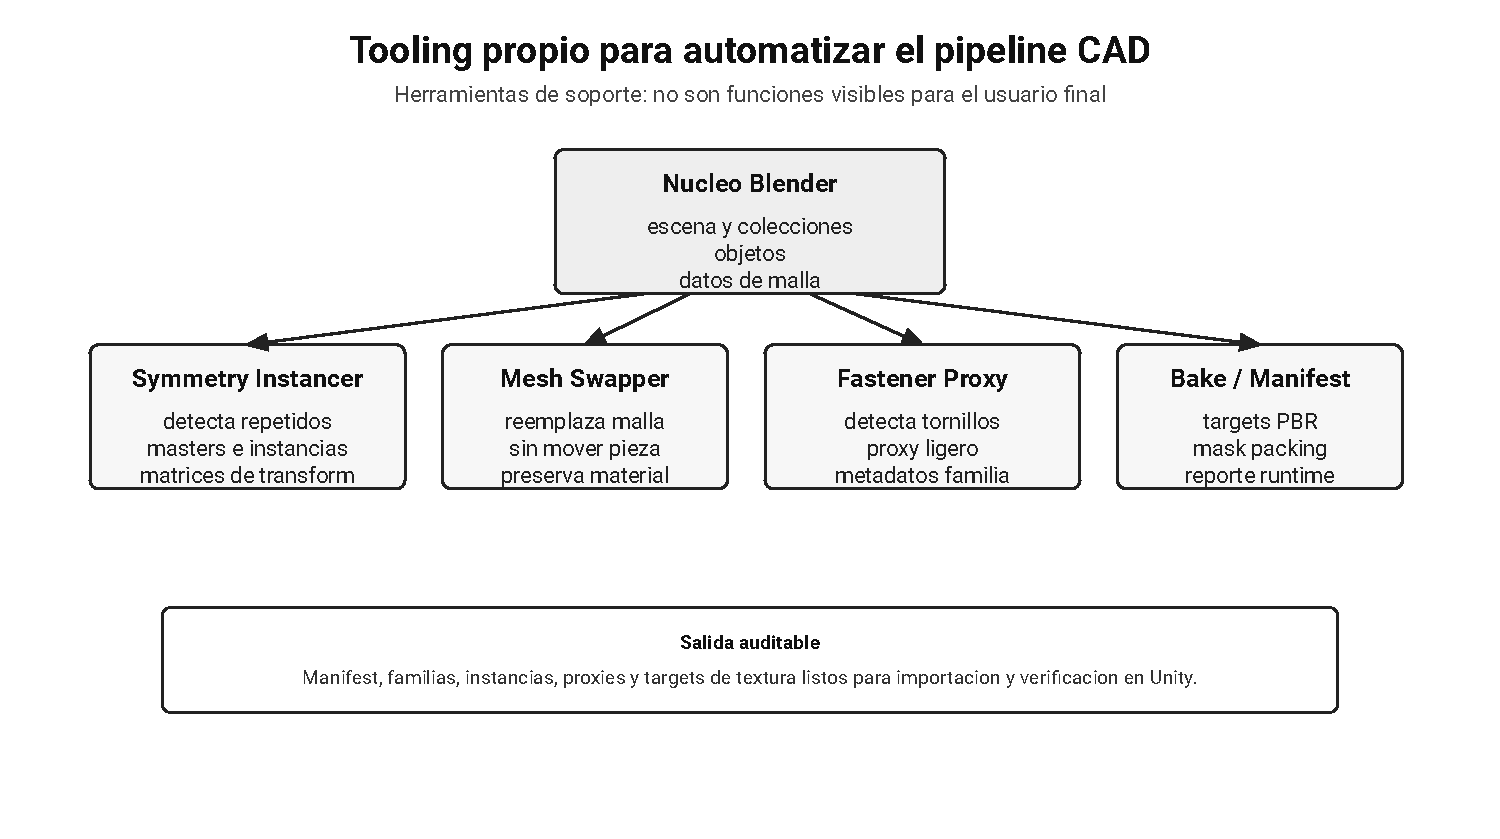
\includegraphics[width=\textwidth,height=0.58\textheight,keepaspectratio]{figures/chapter4/fig_4_addons_pipeline.pdf}
    \par\vspace{0.5\baselineskip}
    \apanote{La figura resume el soporte técnico de automatización del pipeline; no representa funciones visibles para usuarios finales de la aplicación. Elaboración propia.}
\end{figure}

La Figura \ref{fig:evidencia_bake_uv_fasteners_runtime} muestra el estado de alta resolución importado mediante STEPper y utilizado como fuente para el bake. Se presenta con vista sombreada y \textit{wireframe} apilados para conservar el ancho de página sin perder legibilidad. Después, la Figura \ref{fig:evidencia_malla_optimizada_cap4} muestra la malla optimizada usada como referencia del cierre geométrico, también con su lectura \textit{wireframe}.

\begin{figure}[p]
    \caption{Modelo de alta resolución usado como fuente de bake.}
    \label{fig:evidencia_bake_uv_fasteners_runtime}
    \centering
    \includegraphics[width=\textwidth,height=0.35\textheight,keepaspectratio]{figures/screenshots_contextual/fig_cad_bake_high_shaded_full.png}
    \par\vspace{0.35\baselineskip}
    \includegraphics[width=\textwidth,height=0.35\textheight,keepaspectratio]{figures/screenshots_contextual/fig_cad_bake_high_wireframe_full.png}
    \par\vspace{0.5\baselineskip}
    \apanote{La vista sombreada y su equivalente \textit{wireframe} evidencian la densidad geométrica usada como fuente de bake frente al activo optimizado. Elaboración propia.}
\end{figure}

\begin{figure}[p]
    \caption{Malla optimizada del dron después del cierre geométrico.}
    \label{fig:evidencia_malla_optimizada_cap4}
    \centering
    \includegraphics[width=\textwidth,height=0.35\textheight,keepaspectratio]{figures/screenshots_contextual/fig_cad_bake_low_shaded_full.png}
    \par\vspace{0.35\baselineskip}
    \includegraphics[width=\textwidth,height=0.35\textheight,keepaspectratio]{figures/screenshots_contextual/fig_cad_bake_low_wireframe_full.png}
    \par\vspace{0.5\baselineskip}
    \apanote{La captura muestra el activo optimizado usado como referencia visual para el cierre del pipeline, con geometría reducida y lectura \textit{wireframe} de la malla final. Elaboración propia.}
\end{figure}

\subsubsection{Evolución de la estrategia de LOD y migración técnica evaluada}

La planificación inicial contemplaba generar LODs manuales desde Blender, exportarlos por jerarquía y configurarlos mediante grupos tradicionales. Esa estrategia sigue siendo válida conceptualmente: reducir triángulos en mallas lejanas disminuye trabajo de render y ayuda a controlar el presupuesto visual. Sin embargo, la investigación técnica del proyecto llevó a evaluar rutas nativas de \textit{Mesh LOD} dentro del ecosistema Unity 6.x para reducir mantenimiento manual si el cierre del pipeline lo justifica.

Cabe precisar que la adopción plena de una ruta nativa de LOD no se documenta como cambio cerrado de la build. Lo defendible académicamente es explicarla como una decisión técnica evaluada: podría reducir la complejidad de mantenimiento frente a LODs manuales por pieza, alinear mejor el reimport final con un workflow nativo de motor y minimizar retrabajo si el cierre del pipeline exige nuevas iteraciones sobre la geometría (véase la Figura \ref{fig:lod_migration_evaluada}).

\begin{figure}[htbp]
    \caption[Evolución de la estrategia de LOD]{Evolución de la estrategia de LOD: de planificación manual a ruta nativa evaluada.}
    \label{fig:lod_migration_evaluada}
    \centering
    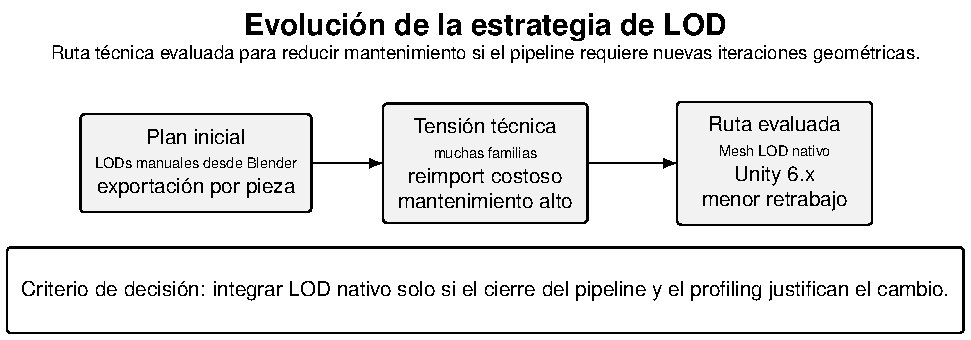
\includegraphics[width=\textwidth,height=0.58\textheight,keepaspectratio]{figures/chapter4/fig_4_lod_migration.pdf}
    \par\vspace{0.5\baselineskip}
    \apanote{La figura documenta una evolución de planeación técnica desde LODs manuales hacia una ruta nativa evaluada dentro del ecosistema Unity. Elaboración propia.}
\end{figure}

\subsection{UX/UI, diseño visual y enfoque \textit{mobile-first}}

El diseño de la interfaz no fue una capa visual independiente de la arquitectura, sino una capa de decisión con respaldo teórico y consecuencias directas sobre la comprensión del ensamblaje. La versión con sustento de diseño mejor fundamentado es la interfaz \textit{mobile-first}. La aplicación en escritorio existe, funciona y se mantiene correcta para uso y demostración; sin embargo, no fue re-diseñada con el mismo nivel de rigor sistémico específico para \textit{desktop}. Por limitaciones de tiempo, la versión de escritorio se conservó como una adaptación funcional del layout móvil (véase la Figura \ref{fig:ui_mobile_desktop_compare}).

La interfaz móvil se apoyó en varios principios convergentes:
\begin{itemize}
    \item jerarquía visual clara para separar navegación primaria, acciones de modo y detalle contextual (Norman, 2013);
    \item agrupación por proximidad, similitud y continuidad para evitar dispersión visual en paneles y tarjetas (Wertheimer, 1923; Köhler, 1929);
    \item soporte a la lectura técnica mediante color, contraste y consistencia visual (Ware, 2012);
    \item control de navegación y selección en entornos 3D con foco en orientación y reducción de fricción operativa (Bowman et al., 2004; Darken \& Sibert, 1996).
\end{itemize}

En la práctica, estas decisiones se tradujeron en una barra inferior persistente de modos, un \textit{bottom sheet} como contenedor principal de detalle, tarjetas de acción compactas y un flujo que minimiza los cambios bruscos de contexto (como se detalla en la Tabla \ref{tab:criterios_uix_mobile_first} y se ilustra en las Figuras \ref{fig:ui_evolution_mobile_first}, \ref{fig:ui_mobile_desktop_compare} y \ref{fig:ui_explore_mobile_pc}).

\begin{table}[H]
    \caption{Criterios de diseño aplicados a la UI del prototipo}
    \label{tab:criterios_uix_mobile_first}
    \centering
    \small
    \begin{tabular}{p{3.2cm}p{4.8cm}p{6.0cm}}
        \hline
        \textbf{Criterio} & \textbf{Aplicación en la app} & \textbf{Interpretación} \\ \hline
        Jerarquía visual & Separación entre Hero, navegación inferior, modos y ficha inferior. & Permite que el usuario identifique el flujo principal sin depender de menús complejos. \\
        Diseño \textit{mobile-first} & Barra inferior, \textit{bottom sheet}, tarjetas táctiles y scroll elástico. & Es la capa de UI con respaldo teórico más consistente del proyecto. \\
        Adaptación a escritorio & Reacomodo funcional del layout móvil sobre una pantalla más amplia. & Es utilizable para demostración y revisión técnica, pero no corresponde a un sistema de diseño de escritorio plenamente desarrollado. \\
        Consistencia cromática y de estados & Paleta contenida, retroalimentación de selección y lectura por modos. & Refuerza la comprensión del sistema y evita ruido visual innecesario durante la inspección. \\ \hline
    \end{tabular}
    \par\vspace{0.5\baselineskip}
    \apanote{Esta tabla evita presentar la versión de escritorio como si hubiera recibido el mismo nivel de diseño sistémico específico que la interfaz móvil. Elaboración propia.}
\end{table}

\begin{figure}[htbp]
    \caption{Evolución de la interfaz hacia el enfoque \textit{mobile-first}.}
    \label{fig:ui_evolution_mobile_first}
    \centering
    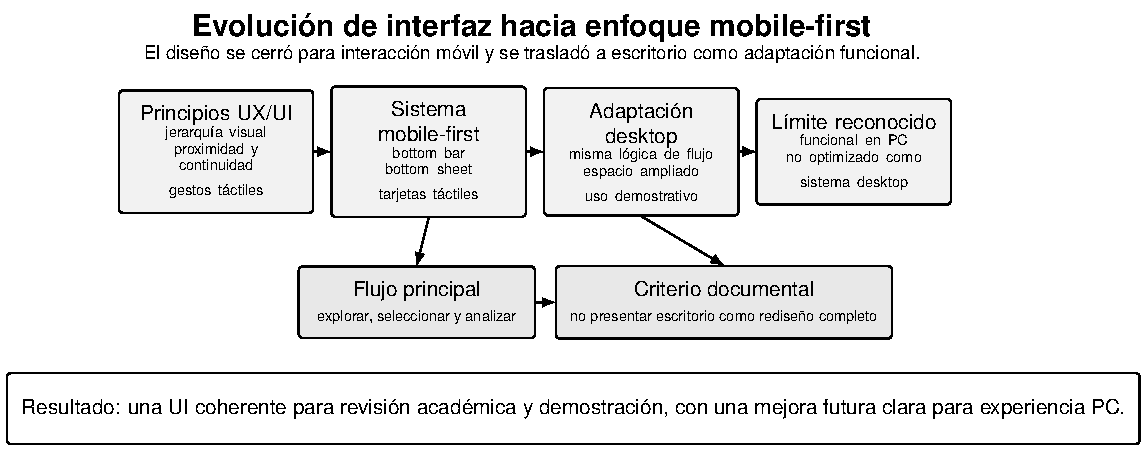
\includegraphics[width=\textwidth,height=0.58\textheight,keepaspectratio]{figures/chapter4/fig_4_ui_evolution_mobile_first.pdf}
    \par\vspace{0.5\baselineskip}
    \apanote{Diagrama editorial de decisiones de interfaz que separa el diseño \textit{mobile-first} de su adaptación funcional a escritorio. Elaboración propia.}
\end{figure}

\begin{figure}[htbp]
    \caption{Hero móvil y adaptación funcional a escritorio.}
    \label{fig:ui_mobile_desktop_compare}
    \centering
    \includegraphics[width=\textwidth,height=0.48\textheight,keepaspectratio]{figures/screenshots_contextual/fig_ui_hero_mobile_pc.png}
    \par\vspace{0.5\baselineskip}
    \apanote{La comparación muestra el Hero en escritorio junto a su versión móvil, evidenciando que la versión desktop opera como adaptación funcional del diseño \textit{mobile-first}. Elaboración propia.}
\end{figure}

\begin{figure}[htbp]
    \caption{Explore móvil y adaptación funcional a escritorio.}
    \label{fig:ui_explore_mobile_pc}
    \centering
    \includegraphics[width=\textwidth,height=0.48\textheight,keepaspectratio]{figures/screenshots_contextual/fig_ui_explore_mobile_pc.png}
    \par\vspace{0.5\baselineskip}
    \apanote{La comparación ubica la vista de exploración dentro del canvas 3D de la app en escritorio y móvil, conservando el mismo flujo de navegación y lectura del modelo. Elaboración propia.}
\end{figure}

\begin{figure}[htbp]
    \caption{Acceso a información de pieza y panel contextual.}
    \label{fig:ui_info_panel}
    \centering
    \includegraphics[width=\textwidth,height=0.78\textheight,keepaspectratio]{figures/screenshots_contextual/fig_ui_info_panel.png}
    \par\vspace{0.5\baselineskip}
    \apanote{La lámina muestra la pestaña que abre el panel de información y el panel contextual de pieza; se presenta como acercamiento de interfaz, no como captura completa de pantalla móvil. Elaboración propia.}
\end{figure}

\subsubsection{Ficha inferior, panel de información y jerarquía de selección}

La ficha inferior no funciona como un panel lateral genérico ni como un contenedor decorativo. En la arquitectura de la build final, el \textit{bottom sheet} es la superficie principal de información contextual. Su controlador asociado, \texttt{UIDetailsSheet}, sincroniza la selección activa con el nombre visible de la pieza, la barra de previsualización, el foco de cámara y los bloques de información de identificación, especificaciones y ensamblaje.

Esta capa es relevante porque la selección del modelo no opera como una lista plana de objetos. El sistema puede resolver una interacción sobre cuatro niveles de lectura: \textbf{pieza madre}, cuando la selección corresponde al conjunto principal; \textbf{subpieza}, cuando el usuario entra a una geometría interna o nivel más fino del conjunto; \textbf{grupo de hotspot}, cuando la selección nace desde un marcador y representa una zona funcional; y \textbf{fastener}, cuando el objetivo es un sujetador individual o modular. En cada caso, la ficha inferior debe presentar la información coherente con el nivel seleccionado.

La misma jerarquía afecta otros subsistemas de la interfaz. El resaltado visual, el recentrado de cámara, el aislamiento y la apertura de la ficha deben compartir el mismo contexto semántico. De lo contrario, el usuario podría seleccionar una subpieza, pero recibir datos de una pieza madre, o activar un aislamiento que no corresponde al elemento descrito. Por esa razón, la ficha inferior se documenta como puente entre geometría, datos y comprensión técnica del ensamblaje.

\subsubsection{Sistema de iconos procedurales y microinteracciones}

Una decisión distintiva del proyecto fue evitar un sistema de iconos basado en texturas o sprites tradicionales y reemplazarlo por iconografía procedural generada en código. La implementación actual usa UI Toolkit con \texttt{Painter2D} y \texttt{MeshGenerationContext} para dibujar trayectorias vectoriales y animarlas mediante una física ligera tipo resorte en \texttt{ProceduralIconBase}. Esta estrategia permitió conservar nitidez vectorial, evitar hojas de sprites y mantener control fino sobre \textit{hover}, \textit{press} y respiración visual de los botones, dentro del mismo sistema de UI runtime (Unity Technologies, 2024d).

En términos conceptuales, el sistema evolucionó desde un plan inicial de iconografía SVG hacia una suite procedural escrita en C\#. Los iconos de \texttt{Home}, \texttt{Reset}, \textit{Inspect}, \texttt{Cut}, \texttt{Explode}, \texttt{Filter}, \texttt{Isolate}, \texttt{Power}, \texttt{Shaders}, \textit{Studio} y otros botones ya existen como clases independientes, y su microinteracción se apoya en desplazamientos, escalados, rotaciones o separaciones controladas por una función \texttt{SpringFloat}. En consecuencia, el trabajo visual del proyecto no se limita a elegir íconos: incorpora geometría procedural, interpolación amortiguada y coherencia entre metáfora visual y función interactiva. La Figura \ref{fig:iconos_microinteracciones} resume esta cadena entre dibujo vectorial, clase base procedural, microinteracción y botones visibles.

\begin{figure}[htbp]
    \caption[Iconos procedurales y microinteracciones]{Sistema de iconos procedurales y microinteracciones implementadas en código.}
    \label{fig:iconos_microinteracciones}
    \centering
    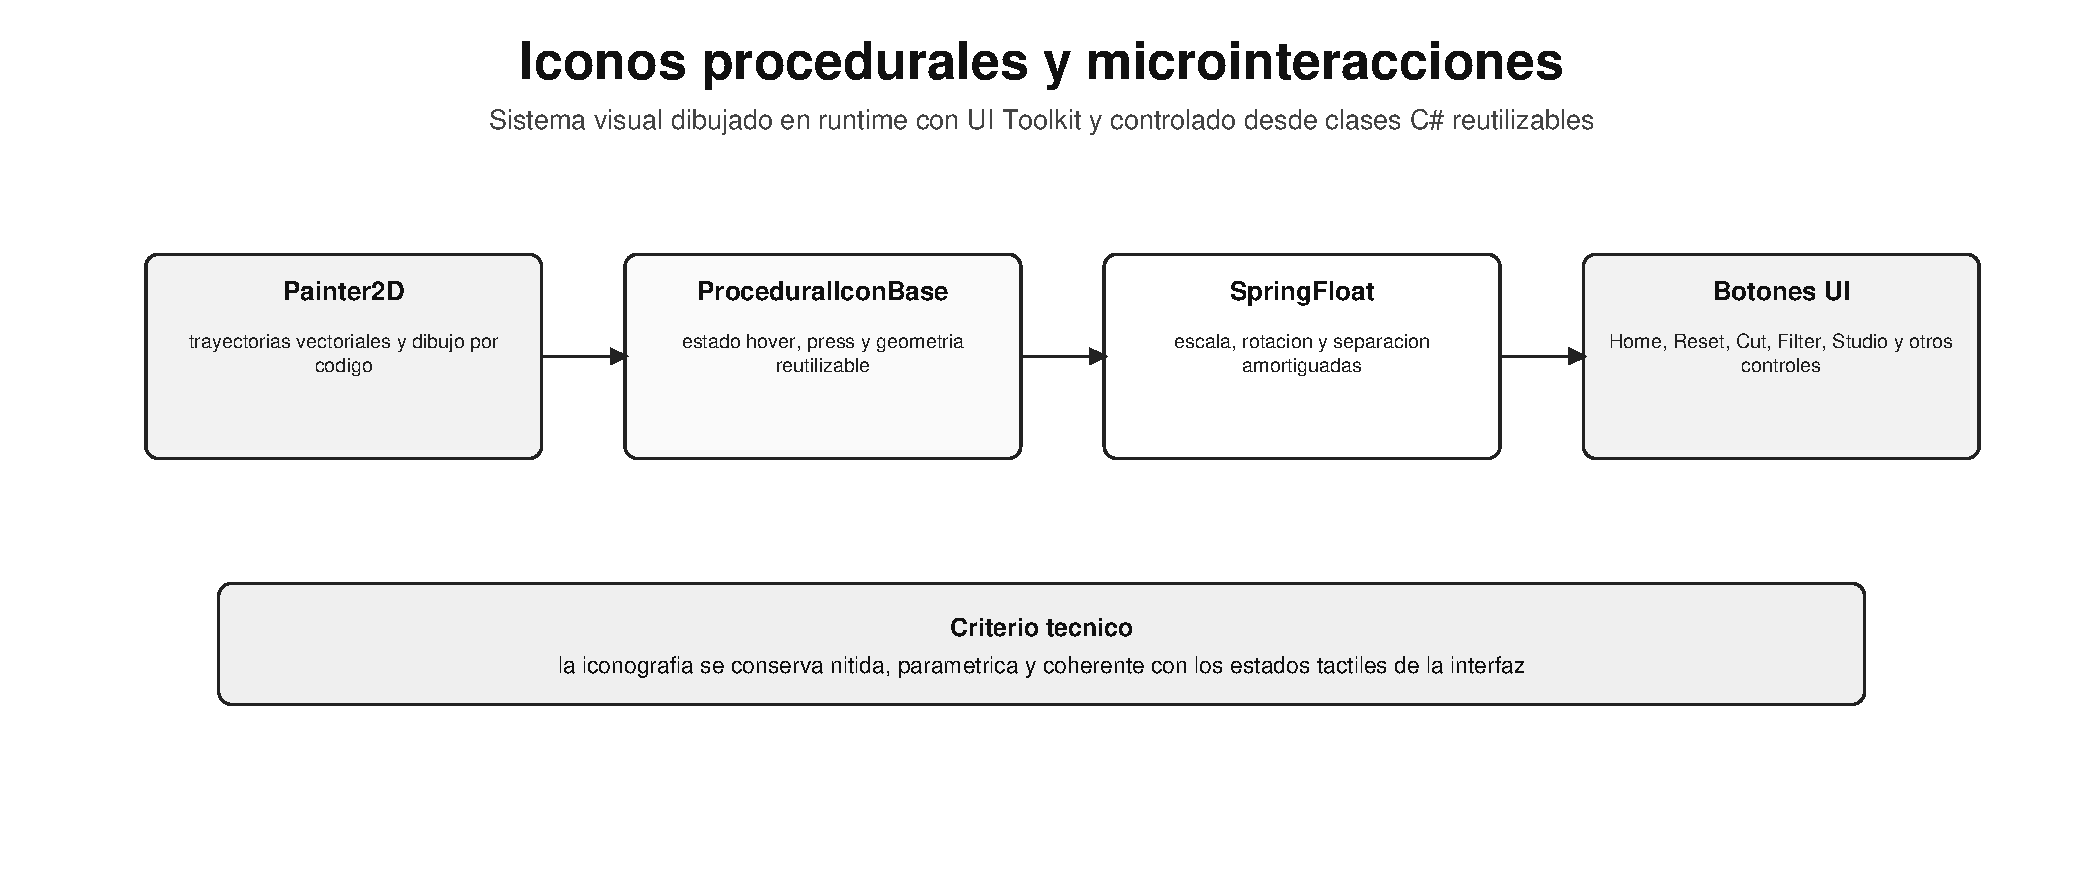
\includegraphics[width=\textwidth,height=0.44\textheight,keepaspectratio]{figures/chapter4/fig_4_iconos_microinteracciones.pdf}
    \par\vspace{0.5\baselineskip}
    \apanote{El diagrama resume la arquitectura de implementación de los iconos procedurales y sus estados interactivos dentro de UI Toolkit. Elaboración propia.}
\end{figure}

\subsubsection{Onboarding procedural y ayuda contextual}

Además del sistema de iconos, el proyecto incorporó un subsistema de onboarding de primer uso para explicar controles, menús y microinteracciones sin depender de medios prerenderizados. La necesidad surgió porque la app no se limita a navegación 3D básica: combina selección jerárquica, \textit{bottom sheet}, menús de inspección y análisis, sliders, modos visuales y variaciones entre escritorio y móvil. En una primera lectura, esa densidad de interacción podía elevar la fricción de entrada si el usuario no recibía una guía integrada al propio producto.

La ruta inicialmente considerada consistía en usar GIFs o clips por tarjeta. Sin embargo, esa opción agregaba peso, duplicaba mantenimiento y se desacoplaba con facilidad del estado real de la interfaz. La solución ejecutada fue un renderer procedural en runtime, implementado sobre \texttt{Painter2D} mediante \texttt{OnboardingAnimationView}, sincronizado por \texttt{OnboardingController} con \texttt{copy}, \textit{cues}, cambio de plataforma y estado del overlay. En lugar de reproducir video, cada tarjeta dibuja actor de interacción, objetivo y respuesta del sistema usando el mismo lenguaje visual del resto de la UI.

La versión actual cubre \textbf{15 tarjetas} y dos variantes de actor: \textbf{desktop} con cursor, botones de mouse, rueda y anillos de click; y \textbf{mobile} con \textit{tap}, \textit{ripple}, \textit{drag} y \textit{pinch} abstractos. Esta arquitectura permitió explicar \texttt{Navigate}, \texttt{Select / Deselect}, \texttt{Part Info}, \textit{Inspect}, \textit{Analyze}, \textit{Studio} y sus subacciones sin recurrir a spritesheets, SVG runtime o videos embebidos. En consecuencia, el onboarding opera como una extensión del sistema de UI procedural, no como un recurso externo agregado al final del proyecto. La Figura \ref{fig:onboarding_runtime} sintetiza la relación entre controlador, tarjetas, vista procedural y variantes de actor por plataforma, mientras que las Figuras \ref{fig:evidencia_tarjetas_onboarding_runtime}, \ref{fig:evidencia_tarjetas_onboarding_runtime_ii}, \ref{fig:evidencia_tarjetas_onboarding_runtime_iii}, \ref{fig:evidencia_tarjetas_onboarding_runtime_iv} y \ref{fig:evidencia_tarjetas_onboarding_runtime_v} muestran las tarjetas visibles integradas en la build en grupos de tres.

\begin{figure}[htbp]
    \caption{Onboarding procedural de primer uso integrado al runtime.}
    \label{fig:onboarding_runtime}
    \centering
    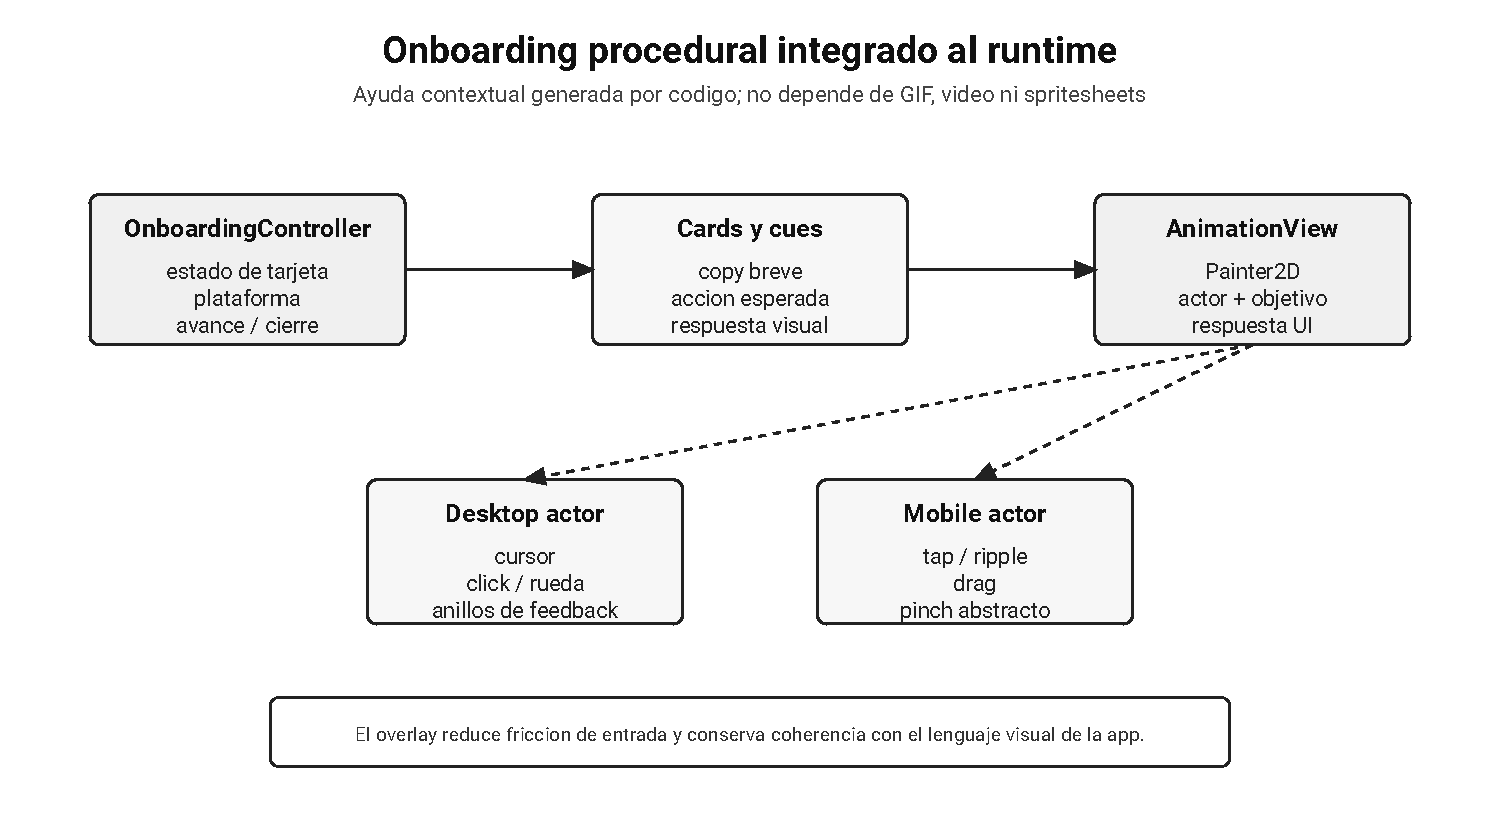
\includegraphics[width=\textwidth,height=0.58\textheight,keepaspectratio]{figures/chapter4/fig_4_onboarding_runtime.pdf}
    \par\vspace{0.5\baselineskip}
    \apanote{El diagrama resume la arquitectura de ayuda contextual generada por código; no depende de GIF, video ni spritesheets. Elaboración propia.}
\end{figure}

\begin{figure}[htbp]
    \caption{Tarjetas del onboarding procedural: navegación, selección e información.}
    \label{fig:evidencia_tarjetas_onboarding_runtime}
    \centering
    \includegraphics[width=0.88\textwidth,height=0.58\textheight,keepaspectratio]{figures/screenshots_contextual/fig_tutorial_cards_01.png}
    \par\vspace{0.5\baselineskip}
    \apanote{De izquierda a derecha se presentan las tarjetas de navegación, selección/deselección e información de pieza. Elaboración propia.}
\end{figure}

\begin{figure}[htbp]
    \caption{Tarjetas del onboarding procedural: inspección, hotspots y aislamiento.}
    \label{fig:evidencia_tarjetas_onboarding_runtime_ii}
    \centering
    \includegraphics[width=0.88\textwidth,height=0.58\textheight,keepaspectratio]{figures/screenshots_contextual/fig_tutorial_cards_02.png}
    \par\vspace{0.5\baselineskip}
    \apanote{De izquierda a derecha se presentan las tarjetas de \textit{Inspect}, pines/hotspots y aislamiento. Elaboración propia.}
\end{figure}

\begin{figure}[htbp]
    \caption{Tarjetas del onboarding procedural: energía, análisis y corte.}
    \label{fig:evidencia_tarjetas_onboarding_runtime_iii}
    \centering
    \includegraphics[width=0.88\textwidth,height=0.58\textheight,keepaspectratio]{figures/screenshots_contextual/fig_tutorial_cards_03.png}
    \par\vspace{0.5\baselineskip}
    \apanote{De izquierda a derecha se presentan las tarjetas de energía/carga, \textit{Analyze} y corte transversal. Elaboración propia.}
\end{figure}

\begin{figure}[htbp]
    \caption{Tarjetas del onboarding procedural: explosión, filtros y Studio.}
    \label{fig:evidencia_tarjetas_onboarding_runtime_iv}
    \centering
    \includegraphics[width=0.88\textwidth,height=0.58\textheight,keepaspectratio]{figures/screenshots_contextual/fig_tutorial_cards_04.png}
    \par\vspace{0.5\baselineskip}
    \apanote{De izquierda a derecha se presentan las tarjetas de vista explosionada, filtros y \textit{Studio}. Elaboración propia.}
\end{figure}

\begin{figure}[htbp]
    \caption{Tarjetas del onboarding procedural: modo de render, ambiente e iluminación.}
    \label{fig:evidencia_tarjetas_onboarding_runtime_v}
    \centering
    \includegraphics[width=0.88\textwidth,height=0.58\textheight,keepaspectratio]{figures/screenshots_contextual/fig_tutorial_cards_05.png}
    \par\vspace{0.5\baselineskip}
    \apanote{De izquierda a derecha se presentan las tarjetas de modo de render, entorno e iluminación. Elaboración propia.}
\end{figure}

\subsection{Arquitectura operativa}

La arquitectura de la aplicación se organiza en cuatro capas de abstracción para garantizar el desacoplamiento entre el diseño de interfaz y la simulación interactiva. La capa de Presentación gestiona el layout responsivo mediante UI Toolkit; la capa de Orquestación coordina la lógica global del flujo de interacción; la capa de Servicios de Escena implementa funciones específicas como corte, explosión y simulación térmica; y la capa de Datos contiene los assets y catálogos serializados del dron (véase la Figura \ref{fig:arquitectura_capas_sistema}).

\begin{figure}[htbp]
    \caption{Arquitectura por capas del sistema.}
    \label{fig:arquitectura_capas_sistema}
    \centering
    \includegraphics[width=0.88\textwidth,height=0.55\textheight,keepaspectratio]{figures/chapter4/fig_4_1.pdf}
    \par\vspace{0.5\baselineskip}
    \apanote{Organización de la aplicación en cuatro capas independientes: presentación (UI), orquestación (manager general y estados), servicios de escena (cámara, corte, explosión y térmico) y datos. Elaboración propia.}
\end{figure}

Para evitar el acoplamiento rígido entre controladores de interfaz y managers de escena, el sistema implementa un bus de eventos (\textit{EventBus}) bajo el patrón de publicación/suscripción. De este modo, eventos como la selección de una pieza o el cambio de modo de renderizado se notifican al bus sin que el emisor conozca la implementación de los receptores, lo que simplifica la extensión del visor (véase la Figura \ref{fig:flujo_eventbus_sistema}).

\begin{figure}[htbp]
    \caption{Flujo de comunicación EventBus bajo el patrón \textit{publish/subscribe}.}
    \label{fig:flujo_eventbus_sistema}
    \centering
    \includegraphics[width=0.88\textwidth,height=0.55\textheight,keepaspectratio]{figures/chapter4/fig_4_2.pdf}
    \par\vspace{0.5\baselineskip}
    \apanote{Diagrama del flujo de mensajes desacoplado entre emisores (UI y managers) y suscriptores de eventos mediante el bus central. Elaboración propia.}
\end{figure}

\FloatBarrier

La secuencia de vistas y el ciclo de vida interactivo están regidos por una máquina de estados finita (\texttt{AppStateMachine}). Esta máquina organiza las transiciones del usuario desde la pantalla inicial, pasando por el onboarding guiado, hasta la exploración libre del modelo 3D y la activación de herramientas analíticas o presets de sombreado (véase la Figura \ref{fig:app_state_machine_sistema}).

\begin{figure}[H]
    \caption{Máquina de estados de la aplicación (\texttt{AppStateMachine}).}
    \label{fig:app_state_machine_sistema}
    \centering
    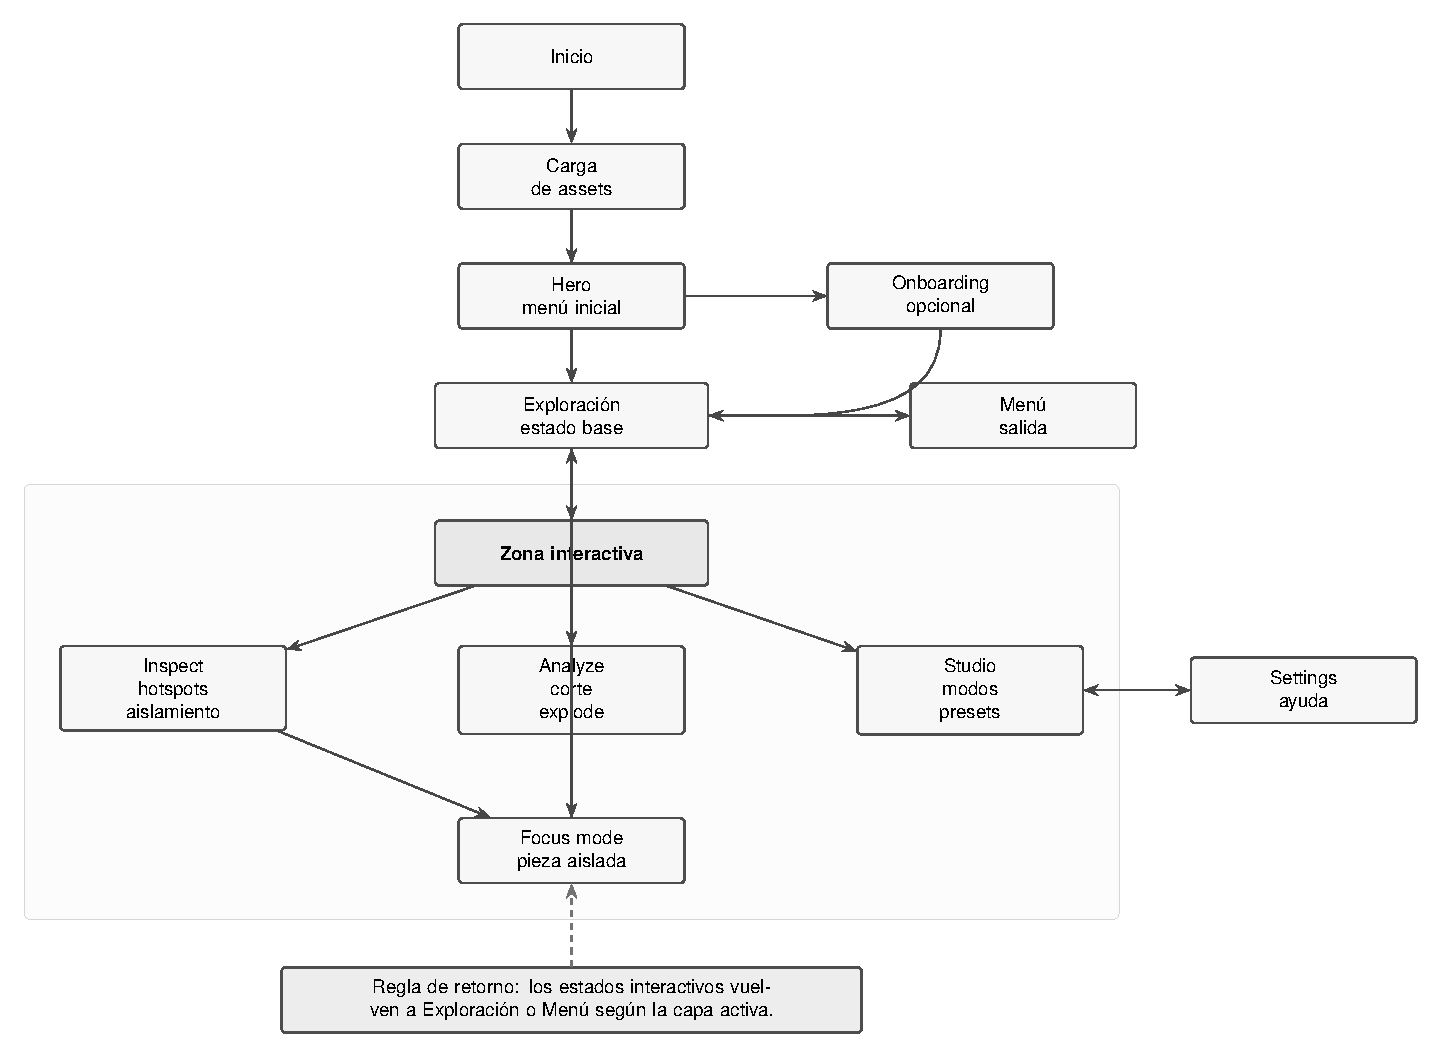
\includegraphics[width=\textwidth,height=0.70\textheight,keepaspectratio]{figures/apa_redesign/fig_apa_app_state_machine.pdf}
    \par\vspace{0.5\baselineskip}
    \apanote{Máquina de estados finitos que controla los estados del visor y las transiciones válidas durante la sesión del usuario. Elaboración propia.}
\end{figure}

\subsubsection{Bootstrap y saneamiento del import}

La escena final depende de dos mecanismos complementarios.

\paragraph{Garantía de managers} Durante la inicialización, \texttt{UIManager} asegura la presencia de los managers mínimos requeridos por el visor: selección, explode, catalogación de runtime, notificaciones, hotspots, clipping, visibilidad, estado del dron y subsistema térmico.

\paragraph{Reparación del modelo importado} \texttt{ImportedDroneRuntimeBinder} corrige la jerarquía del dron importado en runtime. Su trabajo incluye:
\begin{itemize}
    \item resolver anchors por \texttt{id};
    \item reubicar objetos huérfanos de nivel superior o anidados;
    \item sintetizar grupos para fasteners y misceláneos;
    \item reconstruir cachés de \texttt{ExplodedViewManager}, \texttt{PartVisibilityManager}, \texttt{PartCatalogManager}, \texttt{CrossSectionManager}, \texttt{ViewModeManager} y el subsistema térmico.
\end{itemize}

Este saneamiento es decisivo porque traduce la taxonomía académica del proyecto a una escena navegable por la app. Sin esa reparación, la coherencia entre selección, \textit{bottom sheet}, categorías, vistas analíticas y estado térmico se rompería.

La Figura \ref{fig:flujo_dronepartdata_runtime} resume el tránsito de \texttt{DronePartData} desde el asset o catálogo hasta los controladores de interfaz y los servicios de escena.

\begin{figure}[H]
    \caption[Flujo de datos \texttt{DronePartData}]{Flujo de datos \texttt{DronePartData} desde asset y catálogo hasta la interfaz.}
    \label{fig:flujo_dronepartdata_runtime}
    \centering
    \includegraphics[width=\textwidth,height=0.78\textheight,keepaspectratio]{figures/chapter4/fig_4_6.pdf}
    \par\vspace{0.5\baselineskip}
    \apanote{La figura resume la ruta de normalización y consumo de \texttt{DronePartData} en runtime, desde los activos importados y el catálogo hasta los controladores visibles de interfaz y escena. Elaboración propia.}
\end{figure}

\subsection{Flujo visible de la build final}

El flujo principal de uso es:
\begin{center}
\texttt{Hero -> Explore -> selección -> bottom sheet -> Inspect / Analyze / Studio}
\end{center}

\paragraph{Hero} El Hero funciona como puerta de entrada al prototipo (véase la Figura \ref{fig:ui_hero_twinsight_bilingue}). En la versión saneada para cierre, sus textos se anclan al caso real del Holybro X500~V2 y el acceso al repositorio queda cableado desde el submenú \textit{About}. Las pantallas auxiliares del Hero, como \textit{About}, selección de dispositivo y salida de la app, se documentan por separado en la Figura \ref{fig:evidencia_hero_auxiliar_runtime}.

\paragraph{Onboarding y primer uso} En el primer ingreso, y también desde el botón \textit{HELP} del Hero, la app puede abrir un onboarding guiado que resume gestos, selección, paneles, menús, sliders y modos visuales (véase la Figura \ref{fig:onboarding_runtime}). Esta capa cumple una función doble: reduce fricción en el arranque y al mismo tiempo hace visible que la interfaz fue pensada como producto interactivo, no solo como demostración técnica del modelo, la cual se apoya en el sistema de iconos procedurales y microinteracciones de la Figura \ref{fig:iconos_microinteracciones}.

\paragraph{Explore y selección} La vista \textit{Explore} corresponde al canvas 3D principal del modelo (véase la Figura \ref{fig:ui_explore_mobile_pc}). Al seleccionar una pieza, el sistema resalta el objeto y abre una ficha inferior (\textit{bottom sheet}) con información de identificación, especificaciones y ensamblaje (véase la Figura \ref{fig:ui_info_panel}). La selección puede corresponder a una pieza madre, subpieza, grupo de hotspot o fastener; por ello la ficha no solo muestra datos, sino que aclara el nivel de lectura activo. Cuando la selección pertenece a la categoría \texttt{Fasteners}, la ficha usa \texttt{FastenerMetadata} para mostrar familia, métrica, longitud, material, fuente CAD y anchor canónico inferido. La secuencia de hotspot, selección y selección directa se muestra en la Figura \ref{fig:explore_hotspots_selection}; los tres niveles de aislamiento se presentan en la Figura \ref{fig:explore_isolate_sequence}.

\paragraph{Inspect} Reúne hotspots, aislamiento de la pieza seleccionada y control de energía/carga del dron. Su menú principal forma parte de la barra inferior junto a \textit{Analyze} y \textit{Studio} (véase la Figura \ref{fig:evidencia_menus_botones_runtime}), mientras que el control de energía se muestra como acercamiento de botón en la Figura \ref{fig:evidencia_controles_power_cut_runtime}.

\paragraph{Analyze} Integra corte transversal, vista explosionada y filtros por categorías funcionales. La taxonomía activa en esta vista incluye \texttt{SkeletonAirframe}, \texttt{PropulsionSystem}, \texttt{Avionics}, \texttt{SensorsComms}, \texttt{PowerDistribution} y \texttt{Fasteners}. La Figura \ref{fig:evidencia_controles_explode_filter_runtime} muestra los controles de \textit{Explode} y filtros, mientras que la Figura \ref{fig:outputs_analyze_tools_runtime} muestra el efecto visible de \textit{Explode}, \textit{Cut} y \textit{Filter} sobre el modelo.

\paragraph{Studio} Agrupa modos visuales, presets de presentación y control de entorno. El estado base es \textit{Realistic}; la UI visible expone como tarjetas de shader \textit{X-Ray}, \textit{Solid View} o \textit{Solid Color} y \textit{Thermal}. Además, el ciclo de presets de \textit{Studio} permite activar \textit{Studio}, \texttt{Studio Light} y \textit{Blueprint}, junto con controles de ambiente, color y sliders de luz. El panel de \textit{Studio} se presenta como menú de control en la Figura \ref{fig:evidencia_studio_panel_runtime}; los presets visuales se documentan más adelante en las Figuras \ref{fig:studio_presets_blueprint} y \ref{fig:presets_ambiente_color_runtime}.

La separación entre menús, controles y efectos evita mezclar capturas con funciones distintas. Los menús principales de la barra inferior se muestran en la Figura \ref{fig:evidencia_menus_botones_runtime}; las pantallas auxiliares del Hero en la Figura \ref{fig:evidencia_hero_auxiliar_runtime}; los controles de \textit{Power}, \textit{Cut}, \textit{Explode}, \textit{Filter} y \textit{Studio} en las Figuras \ref{fig:evidencia_controles_power_cut_runtime}, \ref{fig:evidencia_controles_explode_filter_runtime} y \ref{fig:evidencia_studio_panel_runtime}; y los efectos directos sobre el modelo en la Figura \ref{fig:outputs_analyze_tools_runtime}.

\begin{figure}[htbp]
    \caption{Menús principales de la barra inferior de la app.}
    \label{fig:evidencia_menus_botones_runtime}
    \centering
    \includegraphics[width=0.88\textwidth,height=0.58\textheight,keepaspectratio]{figures/screenshots_contextual/fig_ui_main_menus.png}
    \par\vspace{0.5\baselineskip}
    \apanote{De izquierda a derecha se presentan los menús principales \textit{Inspect}, \textit{Analyze} y \textit{Studio}. Elaboración propia.}
\end{figure}

Los modos internos no publicados, como \textit{Wireframe} y \textit{Ghosted}, quedan implementados pero ocultos. Por esa razón, no se tratan como capturas del flujo final visible.

La Figura \ref{fig:flujo_seleccion_ui} muestra el recorrido de selección desde el input del usuario hasta la sincronización con el \textit{bottom sheet}.

\begin{figure}[H]
    \caption{Flujo de selección de piezas desde \textit{input} y \textit{raycast} hasta la interfaz.}
    \label{fig:flujo_seleccion_ui}
    \centering
    \includegraphics[width=\textwidth,height=0.78\textheight,keepaspectratio]{figures/chapter4/fig_4_4.pdf}
    \par\vspace{0.5\baselineskip}
    \apanote{El diagrama sintetiza la cadena de selección visible: entrada del usuario, resolución de pieza o subpieza, eventos de escena, resaltado e información presentada en el \textit{bottom sheet}. Elaboración propia.}
\end{figure}

\begin{figure}[htbp]
    \caption{Hero móvil del visor en inglés y español.}
    \label{fig:ui_hero_twinsight_bilingue}
    \centering
    \includegraphics[width=0.88\textwidth,height=0.70\textheight,keepaspectratio]{figures/screenshots_contextual/fig_ui_hero_language.png}
    \par\vspace{0.5\baselineskip}
    \apanote{De izquierda a derecha se presenta el Hero móvil en inglés y en español. Elaboración propia.}
\end{figure}

\begin{figure}[htbp]
    \caption{Pantallas auxiliares del Hero.}
    \label{fig:evidencia_hero_auxiliar_runtime}
    \centering
    \includegraphics[width=0.78\textwidth,height=0.56\textheight,keepaspectratio]{figures/screenshots_contextual/fig_ui_hero_auxiliary.png}
    \par\vspace{0.5\baselineskip}
    \apanote{De izquierda a derecha se muestran las pantallas \textit{About}, selección de dispositivo y salida de la app. Elaboración propia.}
\end{figure}

\begin{figure}[htbp]
    \caption{Controles de energía y corte transversal.}
    \label{fig:evidencia_controles_power_cut_runtime}
    \centering
    \includegraphics[width=0.76\textwidth,height=0.42\textheight,keepaspectratio]{figures/screenshots_contextual/fig_ui_tool_controls_power_cut.png}
    \par\vspace{0.5\baselineskip}
    \apanote{De izquierda a derecha se presentan los acercamientos de control de energía/carga y corte transversal. Elaboración propia.}
\end{figure}

\begin{figure}[htbp]
    \caption{Controles de vista explosionada y filtros.}
    \label{fig:evidencia_controles_explode_filter_runtime}
    \centering
    \includegraphics[width=0.76\textwidth,height=0.42\textheight,keepaspectratio]{figures/screenshots_contextual/fig_ui_tool_controls_explode_filter.png}
    \par\vspace{0.5\baselineskip}
    \apanote{De izquierda a derecha se presentan los acercamientos de vista explosionada y filtros por categoría. Elaboración propia.}
\end{figure}

\begin{figure}[htbp]
    \caption{Panel de control del menú \textit{Studio}.}
    \label{fig:evidencia_studio_panel_runtime}
    \centering
    \includegraphics[width=0.48\textwidth,height=0.58\textheight,keepaspectratio]{figures/screenshots_contextual/fig_ui_studio_panel.png}
    \par\vspace{0.5\baselineskip}
    \apanote{La captura corresponde al menú de \textit{Studio} como panel de controles; no representa el preset visual \textit{Studio Dark}. Elaboración propia.}
\end{figure}

\begin{figure}[htbp]
    \caption{Hotspot y secuencia de selección en \textit{Explore}.}
    \label{fig:explore_hotspots_selection}
    \centering
    \includegraphics[width=0.88\textwidth,height=0.58\textheight,keepaspectratio]{figures/screenshots_contextual/fig_explore_hotspot_selection.png}
    \par\vspace{0.5\baselineskip}
    \apanote{De izquierda a derecha se presenta la selección de hotspot y dos estados de selección directa sobre piezas del modelo. Elaboración propia.}
\end{figure}

\begin{figure}[htbp]
    \caption{Secuencia de aislamiento por niveles en \textit{Inspect}.}
    \label{fig:explore_isolate_sequence}
    \centering
    \includegraphics[width=0.88\textwidth,height=0.58\textheight,keepaspectratio]{figures/screenshots_contextual/fig_explore_isolate_sequence.png}
    \par\vspace{0.5\baselineskip}
    \apanote{De izquierda a derecha se muestran tres niveles de aislamiento aplicados desde el flujo \textit{Inspect}. Elaboración propia.}
\end{figure}

\begin{figure}[htbp]
    \caption{Efectos visibles de \textit{Explode}, \textit{Cut} y filtros sobre el modelo.}
    \label{fig:outputs_analyze_tools_runtime}
    \centering
    \includegraphics[width=0.88\textwidth,height=0.58\textheight,keepaspectratio]{figures/screenshots_contextual/fig_analyze_tool_outputs.png}
    \par\vspace{0.5\baselineskip}
    \apanote{De izquierda a derecha se muestra la vista explosionada, el corte transversal y la aplicación de filtros por categoría. Elaboración propia.}
\end{figure}

\FloatBarrier

\subsection{Sistema de visualización, shaders y entornos}

\texttt{ViewModeManager} implementa siete modos de vista: \textit{Realistic}, \texttt{XRay}, \textit{Blueprint}, \texttt{SolidColor}, \textit{Wireframe}, \textit{Ghosted} y \textit{Thermal}. La UI visible no los expone todos como tarjetas de shader: \textit{X-Ray}, \textit{Solid View}/\textit{Solid Color} y \textit{Thermal} aparecen como modos directos; \textit{Blueprint} se publica mediante el preset de \textit{Studio}; \textit{Wireframe} y \textit{Ghosted} permanecen como capacidades implementadas no visibles en el flujo final.

Para clasificar estas opciones de visualización según su funcionalidad técnica y su acceso en la interfaz, se definió un mapa de modos visuales por propósito (véase la Figura \ref{fig:mapa_modos_visuales_proposito}). Este mapa agrupa las representaciones en realistas, analíticas y de soporte de desarrollo, indicando en qué sección de la UI se expone cada una.

\begin{figure}[H]
    \caption{Mapa de modos visuales por propósito y lugar en la UI.}
    \label{fig:mapa_modos_visuales_proposito}
    \centering
    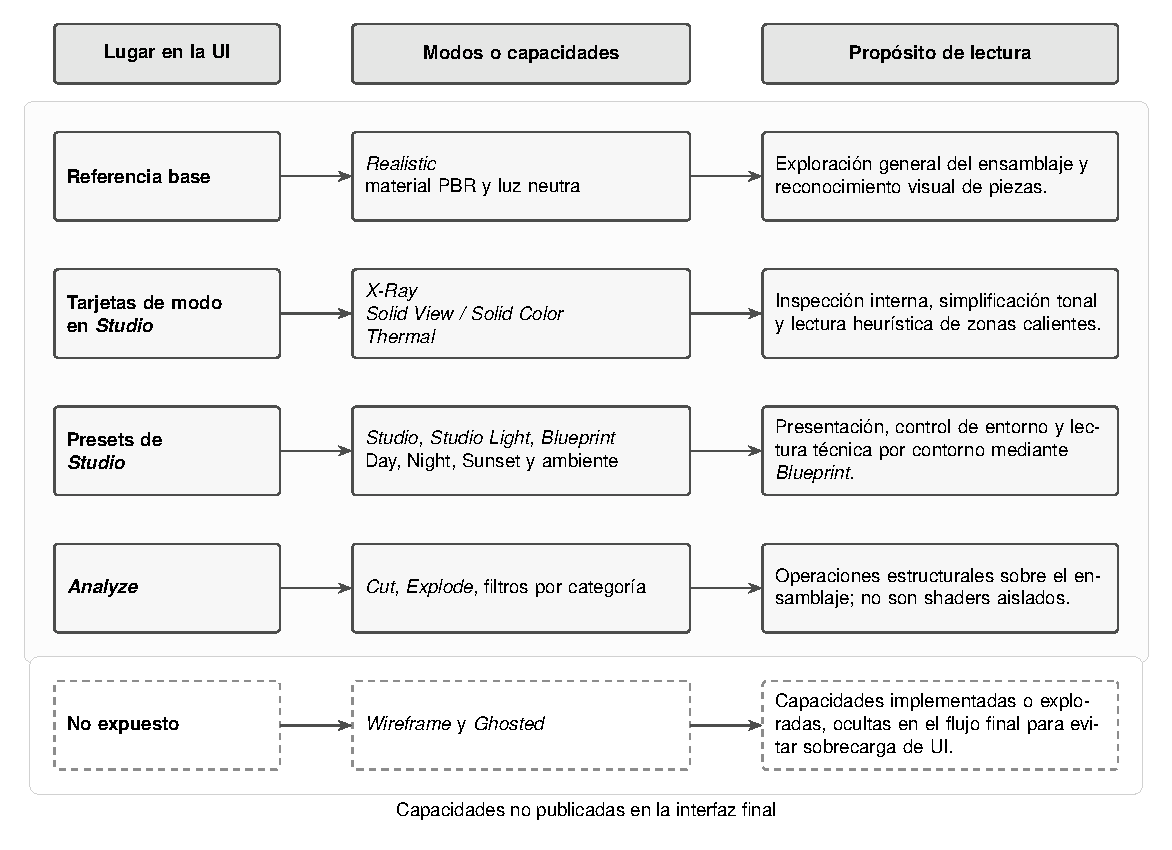
\includegraphics[width=\textwidth,height=0.55\textheight,keepaspectratio]{figures/apa_redesign/fig_apa_mapa_modos_visuales_proposito.pdf}
    \par\vspace{0.5\baselineskip}
    \apanote{Las tarjetas de modo visibles se encuentran dentro de \textit{Studio}: \textit{X-Ray}, \textit{Solid View} y \textit{Thermal} funcionan como modos/shaders directos, mientras que \textit{Studio}, \textit{Studio Light}, \textit{Blueprint} y los ambientes operan como presets de iluminación o apariencia. \textit{Wireframe} y \textit{Ghosted} permanecen como capacidades no publicadas en el flujo final. Elaboración propia.}
\end{figure}

A nivel de renderizado, cada modo interactúa de forma distinta con el pipeline gráfico y los materiales de soporte. La arquitectura del pipeline de shaders discrimina el flujo de datos según el modo de visualización activo, procesando pasadas específicas de contornos, transparencias o gradientes térmicos (véase la Figura \ref{fig:pipeline_shaders_modos}).

\begin{figure}[H]
    \caption[Pipeline de shaders por modo de visualización]{Pipeline de shaders por modo de visualización, distinguiendo entre modos implementados y modos expuestos en la UI final.}
    \label{fig:pipeline_shaders_modos}
    \centering
    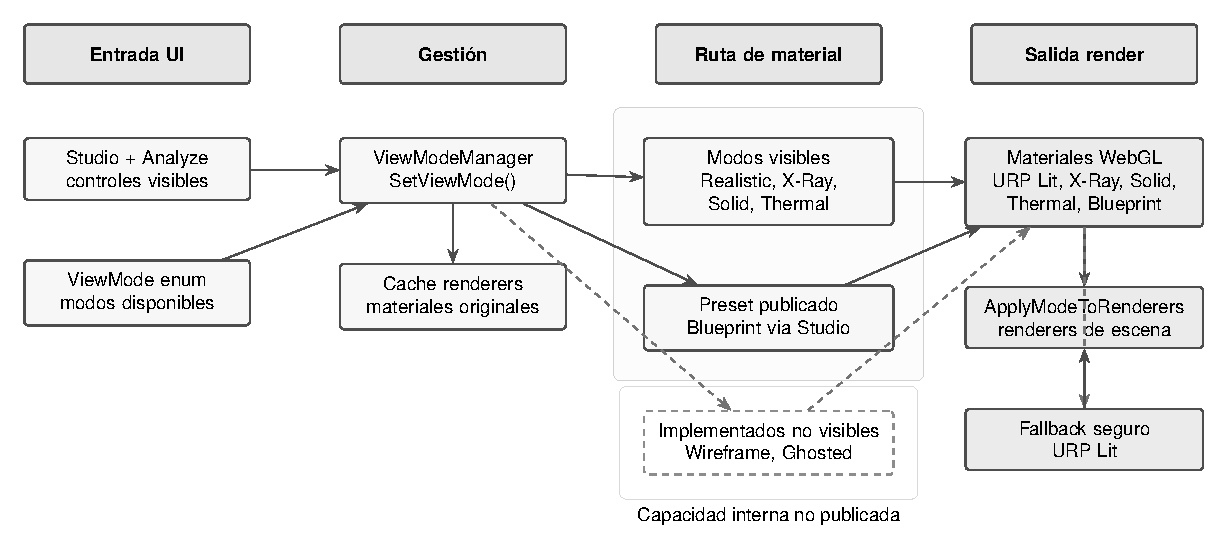
\includegraphics[width=\textwidth,height=0.72\textheight,keepaspectratio]{figures/apa_redesign/fig_apa_pipeline_shaders_modos.pdf}
    \par\vspace{0.5\baselineskip}
    \apanote{Diagrama del flujo de datos de renderizado y lógica de shaders aplicada por el motor para generar cada uno de los modos gráficos expuestos u ocultos. Elaboración propia.}
\end{figure}

\subsubsection{Modo Blueprint y lectura analítica}

El modo \textit{Blueprint} merece una aclaración específica. La UI final no lo publica como tarjeta directa dentro del grupo de shaders, pero sí lo integra en el ciclo de presets de \textit{Studio}. Al activarse desde esa tarjeta, el sistema cambia el modo base a \textit{Blueprint} y aplica una lectura técnica basada en material propio, color de línea, color de fondo, umbral de borde, grilla y detección de contornos (véase la Figura \ref{fig:studio_presets_blueprint}). En términos de diseño visual, este modo se concibió para convertir la escena en una lectura de planos y siluetas técnicas sin perder la posibilidad de inspección 3D. Por ello funciona como puente entre un lenguaje de representación casi diagramático y el modelo navegable en tiempo real.

\subsubsection{Entornos, presets y color base}

La capa de entorno combina dos ciclos. El primero organiza la lectura temporal de iluminación con presets \textit{Day}, \textit{Sunset} y \textit{Night}. El segundo introduce presets de estudio y apariencia general, entre ellos \textit{Studio}, \texttt{Studio Light} y \textit{Blueprint}. Adicionalmente, la UI permite recorrer una base cromática compuesta por blanco, gris, negro, amarillo, naranja, verde, azul, púrpura y rojo. Esta capa fue útil para dos tareas: controlar el contraste visual del modelo y evaluar cómo la interfaz y los iconos procedurales responden a fondos claros u oscuros (como se resume en la Tabla \ref{tab:modos_visuales_publicacion}, que detalla la relación de publicación de cada modo en la UI y su rol visual).

\begin{table}[p]
    \caption{Modos visuales, publicación en UI y lectura técnica}
    \label{tab:modos_visuales_publicacion}
    \centering
    \footnotesize
    \setlength{\tabcolsep}{3pt}
    \renewcommand{\arraystretch}{0.78}
    \begin{tabular}{>{\RaggedRight\arraybackslash}p{2.55cm}>{\RaggedRight\arraybackslash}p{2.35cm}>{\RaggedRight\arraybackslash}p{3.0cm}>{\RaggedRight\arraybackslash}p{5.0cm}}
        \hline
        \textbf{Modo o preset} & \textbf{Estado UI} & \textbf{Rol visual} & \textbf{Interpretación} \\ \hline
        Realistic & Visible & Estado base PBR & Referencia principal del visor para lectura material y navegación general. \\
        X-Ray & Visible & Inspección interna & Aporta transparencia y lectura estructural sin desmontaje completo. \\
        Solid View / Solid Color & Visible & Color plano y contorno & Útil para lectura formal, evaluación de contraste y lectura de siluetas sin textura realista. \\
        Thermal & Visible & Análisis visual guiado por temperatura heurística & Debe documentarse como simulación híbrida, no FEA. \\
        Blueprint & Visible como preset de Studio & Lectura técnico-diagramática & Se activa desde el ciclo de Studio; funciona como preset técnico con líneas, grilla y contornos. \\
        Wireframe & Oculto & Lectura de malla & Debe tratarse como capacidad implementada no publicada. \\
        Ghosted & Oculto & Visualización analítica adicional & Se conserva como capacidad técnica no expuesta. \\
        Day / Sunset / Night & Visible & Variación temporal de ambiente & Afectan contraste, percepción volumétrica y presentación. \\
        Studio / Studio Light / Blueprint & Visible & Presets de estudio, iluminación y lectura técnica & Sirven para presentación, lectura técnica y control visual del modelo. \\ \hline
    \end{tabular}
    \par\vspace{0.5\baselineskip}
    \apanote{La tabla distingue entre tarjetas visibles, presets publicados indirectamente y capacidades ocultas, evitando confundir \textit{Blueprint} con funciones no expuestas como \textit{Wireframe} o \textit{Ghosted}. Elaboración propia a partir del código y de la validación funcional del proyecto.}
\end{table}

La evidencia visual se organiza en grupos pequeños para no mezclar controles con resultados. Los modos directos de render se muestran en la Figura \ref{fig:modes_xray_solid_thermal}; los presets de \textit{Studio}, incluyendo \textit{Blueprint}, se muestran en la Figura \ref{fig:studio_presets_blueprint}; y la variación de entorno/color se muestra en la Figura \ref{fig:presets_ambiente_color_runtime}. Los efectos de \textit{Explode}, \textit{Cut} y \textit{Filter} sobre el modelo se documentaron previamente en la Figura \ref{fig:outputs_analyze_tools_runtime}.

\begin{figure}[htbp]
    \caption{Modos directos de render para inspección visual del ensamblaje.}
    \label{fig:modes_xray_solid_thermal}
    \centering
    \includegraphics[width=\textwidth,height=0.66\textheight,keepaspectratio]{figures/screenshots_contextual/fig_modes_direct_xray_solid_thermal.png}
    \par\vspace{0.5\baselineskip}
    \apanote{De izquierda a derecha: \textit{X-Ray}, \textit{Solid} y \textit{Thermal}. Las capturas se agrupan porque corresponden al mismo panel de modos de render y mantienen proporción de pantalla móvil. Elaboración propia.}
\end{figure}

\begin{figure}[htbp]
    \caption{Presets de \textit{Studio} y lectura \textit{Blueprint}.}
    \label{fig:studio_presets_blueprint}
    \centering
    \includegraphics[width=\textwidth,height=0.66\textheight,keepaspectratio]{figures/screenshots_contextual/fig_modes_studio_presets.png}
    \par\vspace{0.5\baselineskip}
    \apanote{El preset \textit{Blueprint} se activa desde \textit{Studio} y muestra contornos, grilla y lectura técnica sin equivaler al modo oculto \textit{Wireframe}. La lámina también documenta presets de presentación e iluminación del mismo panel. Elaboración propia.}
\end{figure}

\begin{figure}[htbp]
    \caption{Variación de entorno y color base desde \textit{Studio}.}
    \label{fig:presets_ambiente_color_runtime}
    \centering
    \includegraphics[width=0.82\textwidth,height=0.62\textheight,keepaspectratio]{figures/screenshots_contextual/fig_modes_environment_color.png}
    \par\vspace{0.5\baselineskip}
    \apanote{Las capturas ilustran cambios de ambiente y color base que afectan contraste, legibilidad del modelo y lectura de la interfaz sin modificar la geometría. Elaboración propia.}
\end{figure}

\subsection{Modelo matemático operativo del subsistema térmico}

El modo \textit{Thermal} no implementa una simulación FEA ni una solución termodinámica de alta fidelidad. La versión final usa un solver reducido por componentes (\textit{lumped-component model}) coherente con la arquitectura real del código: \texttt{DroneStateController} aporta el factor de carga, \texttt{ThermalSimulationManager} resuelve temperaturas por nodo y \texttt{ThermalViewController} traduce esas temperaturas a bandas visuales para shader y leyenda.

Para cada nodo térmico, la temperatura de equilibrio depende de la carga efectiva del dron. Si la pieza no es fuente de calor, se toma:
\[
T_{eq} = T_{amb}
\]

Para fuentes térmicas, el equilibrio se interpola entre temperatura ambiente, temperatura de hover y temperatura pico según el factor de carga efectivo del sistema. La aproximación temporal hacia ese equilibrio se modela como:
\[
\Delta T_{\text{source}} = \left(T_{eq} - T_{actual}\right)\left(1 - e^{-\Delta t / \tau}\right)w_s
\]
donde $\tau$ es el tiempo de calentamiento configurado para la pieza y $w_s$ es su peso relativo como fuente térmica.

El enfriamiento ambiental se aplica como:
\[
\Delta T_{\text{cooling}} = \left(T_{amb} - T_{actual}\right)\, c_r \, \phi_{\text{exp}} \, \Delta t
\]
donde $c_r$ es la tasa de enfriamiento y $\phi_{\text{exp}}$ el factor de exposición convectiva.

La transferencia entre piezas conectadas por el grafo térmico se aproxima mediante:
\[
\Delta T_{ij} = \left(T_j - T_i\right)\hat{G}_{ij}\Delta t
\]
con un coeficiente de acoplamiento geométrico definido como:
\[
\hat{G}_{ij} = \max\left(0.001,\; s_{ij}\frac{A_{ij}}{L_{ij}}\right)
\]
donde $A_{ij}$ corresponde al área de contacto proxy, $L_{ij}$ a la longitud efectiva del camino térmico y $s_{ij}$ a un factor heurístico de enlace. En consecuencia, el sistema comparte la lógica de una conducción tipo Fourier, pero no debe interpretarse como una conductancia física calibrada en unidades SI.

La trazabilidad matemática del subsistema fue contrastada con el workflow de verificación basado en WolframAlpha utilizado por el proyecto. Dicho audit confirmó tres puntos: la estructura geométrica inspirada en $A/L$ es razonable para el acoplamiento entre nodos, los tiempos de calentamiento del solver están deliberadamente comprimidos frente a valores físicos reales para mantener legibilidad interactiva, y la tasa de enfriamiento por defecto es coherente con esa misma escala temporal acelerada. Por ello, este subsistema debe documentarse como simulación térmica híbrida y heurística, no como FEA en tiempo real.

La Figura \ref{fig:subsistema_termico_hibrido} articula la relación entre el estado del dron, la simulación térmica y la traducción visual del gradiente en la build final. A continuación, la Figura \ref{fig:thermal_bateria_motores_helices} muestra su traducción visual en la interfaz: un gradiente heurístico por componentes que orienta la inspección, sin representar termografía medida, FEA ni temperatura calibrada.

\begin{figure}[H]
    \caption{Arquitectura del subsistema térmico híbrido.}
    \label{fig:subsistema_termico_hibrido}
    \centering
    \includegraphics[width=\textwidth,height=0.78\textheight,keepaspectratio]{figures/chapter4/fig_4_7.pdf}
    \par\vspace{0.5\baselineskip}
    \apanote{La figura ubica el modo \textit{Thermal} como capa visual heurística por componentes, conectada al estado del dron y a un grafo térmico simplificado; no representa FEA, termografía ni temperatura real calibrada. Elaboración propia.}
\end{figure}

\begin{figure}[htbp]
    \caption{Lectura visual del modo \textit{Thermal} en la build final.}
    \label{fig:thermal_bateria_motores_helices}
    \centering
    \includegraphics[width=0.52\textwidth,height=0.60\textheight,keepaspectratio]{figures/screenshots_contextual/fig_thermal_single.png}
    \par\vspace{0.5\baselineskip}
    \apanote{La captura muestra la convención visual usada para diferenciar componentes calientes y piezas pasivas dentro del modelo térmico heurístico. La leyenda orienta la lectura del gradiente sin representar termografía medida ni simulación FEA. Elaboración propia.}
\end{figure}

Para facilitar la comprensión del alcance y la organización del software interactivo desarrollado, los diferentes componentes del visor 3D se agrupan según su nivel de visibilidad y madurez en la build final (véase la Tabla \ref{tab:inventario_modulos_integracion}).

\subsection{Matriz de estado funcional}

\subsubsection{Expuesto en UI final}

\begin{itemize}
    \item Hero y navegación principal;
    \item selección de piezas y \textit{bottom sheet};
    \item hotspots;
    \item isolate;
    \item power y slider de carga;
    \item explode;
    \item cross-section;
    \item filtros por categoría;
    \item modos visuales \textit{X-Ray}, \textit{Solid View}/\textit{Solid Color} y \textit{Thermal};
    \item presets de \textit{Studio}, incluyendo \textit{Blueprint};
    \item thermal con leyenda visible.
\end{itemize}

\subsubsection{Implementado pero oculto}

\begin{itemize}
    \item \texttt{MeasurementTool};
    \item modos de vista \textit{Wireframe} y \textit{Ghosted} como capacidades implementadas pero no expuestas en la UI final;
    \item parte del flujo térmico avanzado y del clipping extendido.
\end{itemize}

\subsubsection{Código legado o no integrado}

\begin{itemize}
    \item \texttt{PartCatalogUI};
    \item \texttt{SettingsPanel};
    \item \texttt{LoadingController};
    \item partes de \texttt{EnhancedInfoPanel};
    \item suite de ensamblaje, BOM, anotaciones y connections.
\end{itemize}

\begin{table}[p]
    \caption{Inventario sintético de módulos y estado de integración}
    \label{tab:inventario_modulos_integracion}
    \centering
    \footnotesize
    \setlength{\tabcolsep}{3pt}
    \renewcommand{\arraystretch}{0.8}
    \begin{tabular}{>{\RaggedRight\arraybackslash}p{3.05cm}>{\RaggedRight\arraybackslash}p{4.35cm}>{\RaggedRight\arraybackslash}p{2.75cm}>{\RaggedRight\arraybackslash}p{4.2cm}}
        \hline
        \textbf{Categoría} & \textbf{Componentes representativos} & \textbf{Estado} & \textbf{Interpretación} \\ \hline
        Runtime principal & Orquestación UI, selección, explode, clipping, view modes, preset \textit{Blueprint} y térmico & Expuesto o activo en la build final & Se documenta en el cuerpo principal porque soporta el flujo visible y la arquitectura operativa. \\
        Capacidades ocultas & \texttt{MeasurementTool}; modos \textit{Wireframe} y \textit{Ghosted}; clipping extendido; térmico avanzado & Implementado pero oculto & Puede mencionarse como capacidad existente, pero no debe narrarse como funcionalidad publicada al usuario final. \\
        Legado o no integrado & Catálogo legado, \texttt{SettingsPanel}, \texttt{LoadingController}, paneles legacy y suite de ensamblaje & No integrado en el flujo final & Debe permanecer separado como legado, trabajo futuro o evidencia histórica de evolución del proyecto. \\
        Tooling de editor & Wizard de proyecto, auditoría de cobertura y constructor del grafo térmico & Soporte técnico de desarrollo & Es pertinente para la defensa técnica y la trazabilidad del pipeline, aunque no forme parte de la UI publicada. \\ \hline
    \end{tabular}
    \par\vspace{0.5\baselineskip}
    \apanote{Esta tabla resume el criterio usado para separar funciones visibles, funciones ocultas y módulos no integrados, evitando mezclar capacidades de desarrollo con el alcance real de la build final. Elaboración propia a partir del código y de la validación funcional del proyecto.}
\end{table}

Esta separación también asegura la coherencia documental entre la aplicación, los manuales y el presente informe (véase la Figura \ref{fig:coherencia_documental_app_manuales_informe}).

\begin{figure}[H]
    \caption{Coherencia documental entre app, manuales e informe.}
    \label{fig:coherencia_documental_app_manuales_informe}
    \centering
    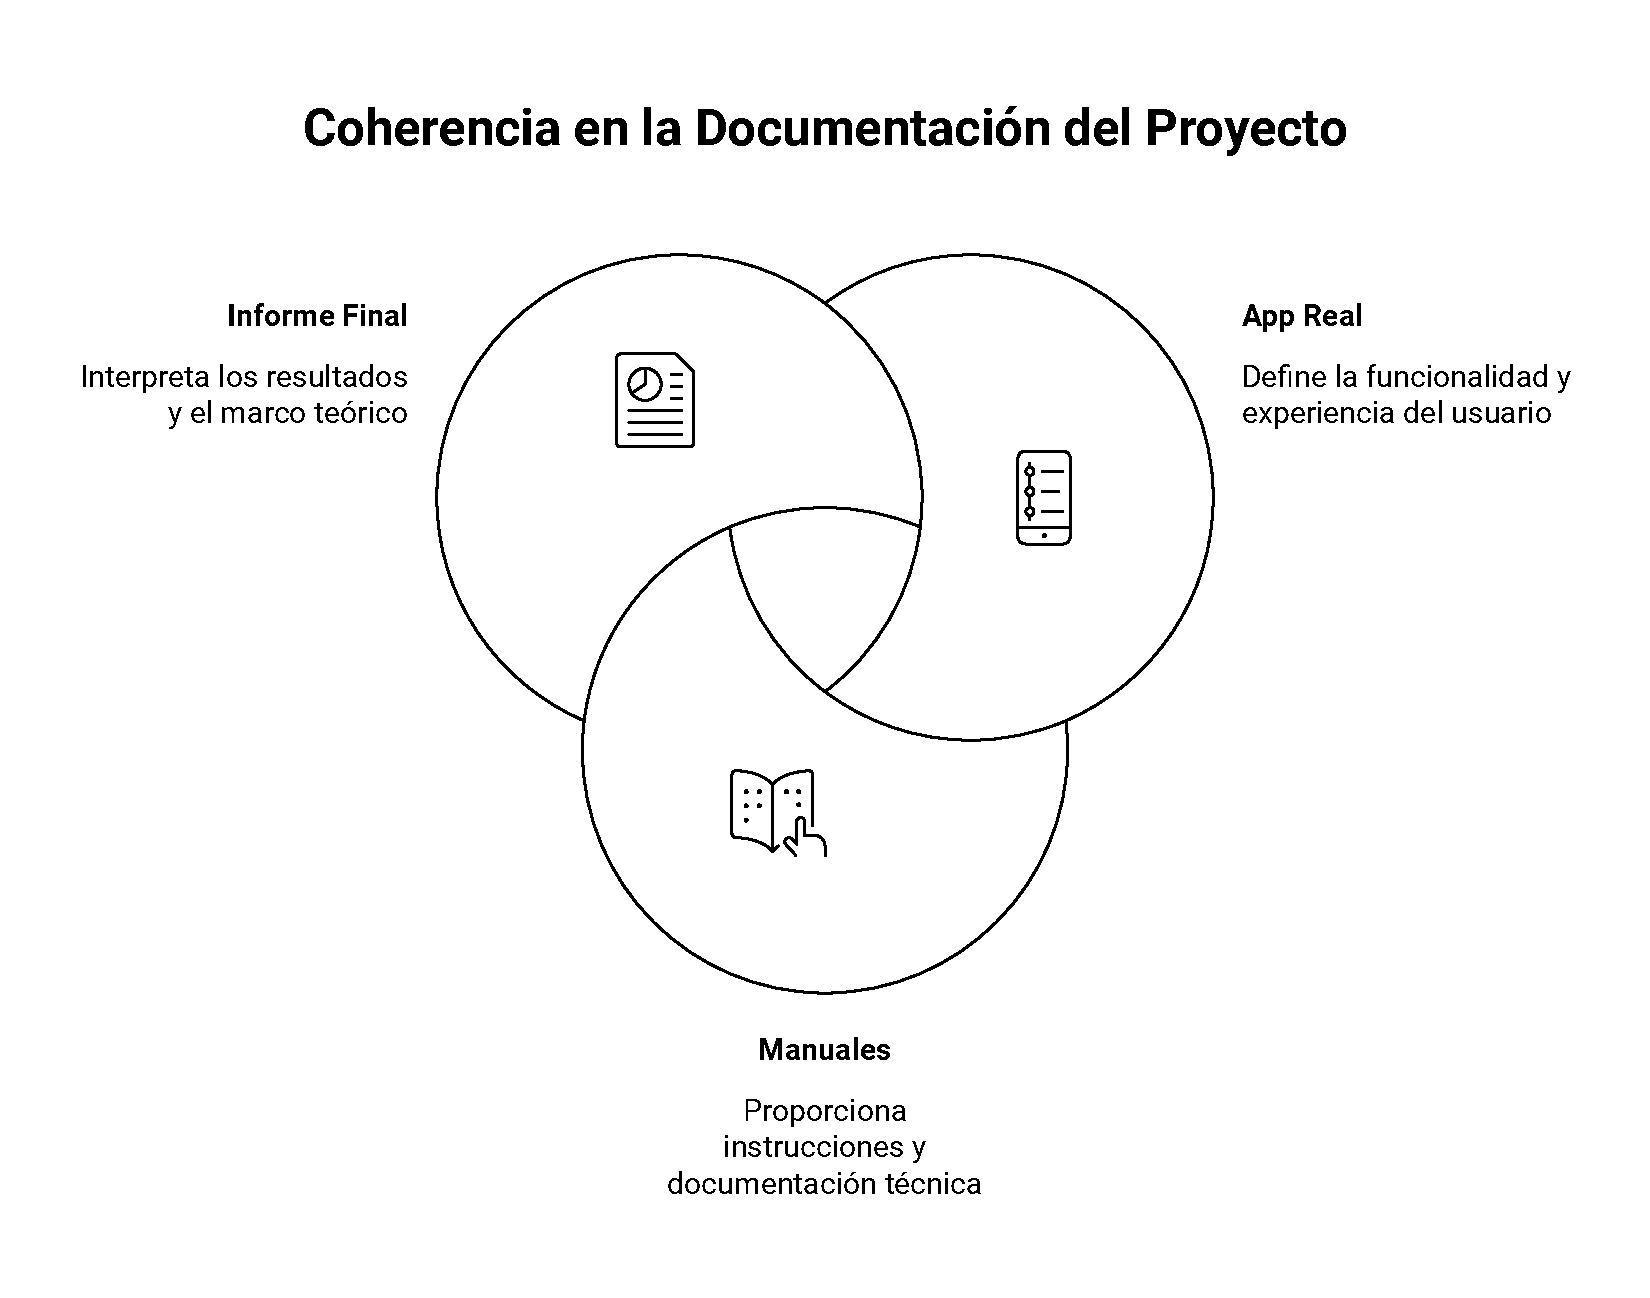
\includegraphics[width=0.86\textwidth,height=0.56\textheight,keepaspectratio]{figures/chapter4/fig_4_coherencia_documental.pdf}
    \par\vspace{0.5\baselineskip}
    \apanote{El criterio de cierre separa funciones visibles, capacidades ocultas, código legado y trabajo futuro para evitar contradicciones entre la build y la documentación. Elaboración propia.}
\end{figure}

\subsection{Tooling de editor, automatización y verificación}

El proyecto conserva herramientas de editor y verificación que sí son defendibles como parte del desarrollo real:
\begin{itemize}
    \item \texttt{ProjectSetupWizard};
    \item \texttt{ImportedDroneCoverageAudit};
    \item \texttt{ThermalContactGraphBuilderWindow};
    \item fixers de configuración y build WebGL.
\end{itemize}

Estas herramientas ayudan a mantener consistencia entre escena, catálogo, render y configuración de despliegue. No forman parte de la UI visible, pero sí del soporte técnico que hizo viable el proyecto.

Para lograr un despliegue viable en navegadores comerciales, el proyecto debió resolver las restricciones de memoria, procesamiento y acceso de la API WebGL. Las mitigaciones técnicas aplicadas incluyen el control estricto del presupuesto geométrico, la compactación de texturas en canales y la configuración óptima del tamaño de la memoria contigua de WebAssembly (véase la Figura \ref{fig:restricciones_webgl_mitigaciones}).

\begin{figure}[H]
    \caption{Restricciones de WebGL y mitigaciones técnicas aplicadas al proyecto.}
    \label{fig:restricciones_webgl_mitigaciones}
    \centering
    \includegraphics[width=0.88\textwidth,height=0.55\textheight,keepaspectratio]{figures/chapter4/fig_4_8.pdf}
    \par\vspace{0.5\baselineskip}
    \apanote{Resumen de los cuellos de botella característicos de la plataforma WebGL (memoria lineal, draw calls, descargas de red) y las correspondientes optimizaciones de Technical Art. Elaboración propia.}
\end{figure}

Una vez generada la build funcional de Unity Web, los archivos resultantes se integran en un pipeline de despliegue continuo alojado en GitHub Pages. Este flujo automatiza la compresión, publicación y verificación rápida del visor interactivo para la validación formativa y QA (véase la Figura \ref{fig:despliegue_artefactos_build}).

\begin{figure}[H]
    \caption{Flujo de despliegue y artefactos desde la build hasta el \textit{hosting} y QA.}
    \label{fig:despliegue_artefactos_build}
    \centering
    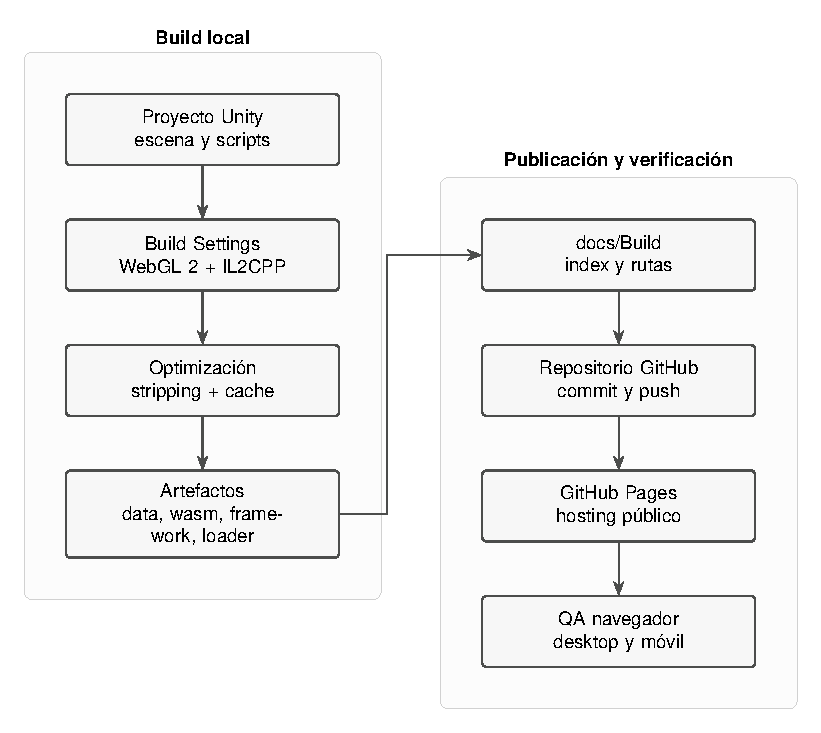
\includegraphics[width=0.82\textwidth,height=0.78\textheight,keepaspectratio]{figures/apa_redesign/fig_apa_despliegue_build_qa.pdf}
    \par\vspace{0.5\baselineskip}
    \apanote{Diagrama de flujo de integración continua, desde el empaquetado de assets hasta la publicación en el servidor de hosting y la evaluación de usuario. Elaboración propia.}
\end{figure}

\subsection{Limitaciones y frentes de cierre}

La build funcional y los ajustes P1/P2 quedan listos para entrega, evaluación y demostración. Los siguientes frentes delimitan el alcance documentado y separan el cierre verificable de las iteraciones futuras:
\begin{enumerate}
    \item conservar como trazabilidad del pipeline la validación del FBX runtime final exportado desde Blender, incluyendo masters, instancias, fasteners primitivos, hélices, hotspots, filtros y grupos;
    \item documentar materiales y texturas finales o, si no entran a la versión publicada, mantenerlos como mejora futura del pipeline visual;
    \item ejecutar rerun de auditorías jerárquicas y de cobertura si se reemplaza la escena o se hace un reimport mayor;
    \item decidir si el audio entra en una iteración posterior o queda como trabajo futuro;
    \item conservar la trazabilidad de métricas cuantitativas de rendimiento, SUS, NASA-TLX Raw y desempeño en tareas reportadas en el capítulo de resultados;
    \item decidir con datos de profiling si una ruta nativa de LOD se integra realmente al cierre del pipeline;
    \item reconocer que la interfaz de escritorio es una adaptación funcional del sistema \textit{mobile-first}, no un sistema desktop rediseñado con el mismo nivel de rigor teórico;
    \item formalizar como trabajo futuro un \textit{twin manifest} por pieza que conecte geometría, categoría, material, función, variables posibles, fallas, repuestos y procedimientos;
    \item mantener telemetría histórica, \textit{live digital shadow}, modo servicio, diagnóstico y simulación calibrada como fases posteriores no implementadas en la build final.
\end{enumerate}

Con estas delimitaciones, el sistema se documenta como funcional y verificable en su flujo principal, con evidencia técnica y de usuario reportada de forma descriptiva en el capítulo 5.

La Figura \ref{fig:herramientas_ensamblaje_proyectadas} deja explícito que el conjunto de herramientas de ensamblaje, BOM, anotaciones y conexiones pertenece a la capa proyectada o no integrada, por lo que no debe confundirse con el flujo visible de la build final.

\begin{figure}[H]
    \caption[Estado de herramientas de ensamblaje]{Estado de herramientas de ensamblaje proyectadas o no integradas por módulo.}
    \label{fig:herramientas_ensamblaje_proyectadas}
    \centering
    \includegraphics[width=0.88\textwidth,height=0.55\textheight,keepaspectratio]{figures/chapter4/fig_4_9.pdf}
    \par\vspace{0.5\baselineskip}
    \apanote{Módulos proyectados en la propuesta original que no fueron integrados en el flujo visible de la build final para acotar el alcance académico. Elaboración propia.}
\end{figure}

\newpage
